\documentclass[a4paper,11pt,oneside]{report}

% Canonical compiler: Tectonic
\usepackage[T1]{fontenc}
\usepackage{lmodern}
\usepackage[inner=30mm,outer=25mm,top=25mm,bottom=27mm,headheight=14pt]{geometry}
\usepackage{microtype}
\usepackage{graphicx}
\usepackage{float}
\usepackage{booktabs}
\usepackage{longtable}
\usepackage{tabularx}
\usepackage{array}
\usepackage{makecell}
\usepackage{amsmath,amssymb}
\usepackage{siunitx}
\usepackage{xcolor}
\usepackage{setspace}
\usepackage{titlesec}
\usepackage{caption}
\usepackage{subcaption}
\usepackage{natbib}
\usepackage{xurl}
\usepackage{fancyhdr}
\usepackage[hidelinks,pdfusetitle]{hyperref}
\usepackage[nameinlink,noabbrev]{cleveref}

\graphicspath{{figures/}{./}}
\sisetup{detect-all,round-mode=places,round-precision=3}
\setstretch{1.04}
\setlength{\parindent}{0pt}
\setlength{\parskip}{0.42em}
\setlength{\emergencystretch}{2em}
\setcounter{tocdepth}{1}
\setlength{\bibsep}{0.35em}
\captionsetup{font=small,labelfont=bf,justification=raggedright,singlelinecheck=false}
\titlespacing*{\chapter}{0pt}{0pt}{16pt}
\titlespacing*{\section}{0pt}{1.6ex plus 0.4ex minus 0.2ex}{0.7ex}
\titlespacing*{\subsection}{0pt}{1.2ex plus 0.3ex minus 0.2ex}{0.5ex}

\definecolor{statusgreen}{HTML}{007A5E}
\definecolor{statusred}{HTML}{B42318}
\definecolor{statusorange}{HTML}{B45309}
\definecolor{statusblue}{HTML}{075985}
\definecolor{statusgray}{HTML}{4B5563}
\newcommand{\passed}{\textcolor{statusgreen}{\textbf{passed}}}
\newcommand{\failed}{\textcolor{statusred}{\textbf{failed}}}
\newcommand{\exploratory}{\textcolor{statusorange}{\textbf{post-hoc}}}
\newcommand{\stopped}{\textcolor{statusblue}{\textbf{stopped}}}
\newcommand{\inconclusive}{\textcolor{statusgray}{\textbf{inconclusive}}}
\newcolumntype{L}[1]{>{\raggedright\arraybackslash}p{#1}}
\newcolumntype{C}[1]{>{\centering\arraybackslash}p{#1}}
\newcolumntype{Y}{>{\raggedright\arraybackslash}X}

\newcommand{\reporttitle}{Passive Sensing Target Validation and Behavioral Forecasting in GLOBEM}
\newcommand{\reportsubtitle}{Research Project Report}
\newcommand{\reportauthor}{Ashutosh Chatterjee}
\newcommand{\reportdate}{16 September 2026}

\pagestyle{fancy}
\fancyhf{}
\fancyhead[L]{\small \nouppercase{\leftmark}}
\fancyhead[R]{\small TU Hamburg Research Project}
\fancyfoot[C]{\thepage}
\renewcommand{\headrulewidth}{0.4pt}
\renewcommand{\footrulewidth}{0pt}
\fancypagestyle{plain}{%
  \fancyhf{}
  \fancyfoot[C]{\thepage}
  \renewcommand{\headrulewidth}{0pt}
}

\crefname{chapter}{Chapter}{Chapters}
\Crefname{chapter}{Chapter}{Chapters}
\crefname{section}{Section}{Sections}
\Crefname{section}{Section}{Sections}
\crefname{figure}{Figure}{Figures}
\Crefname{figure}{Figure}{Figures}
\crefname{table}{Table}{Tables}
\Crefname{table}{Table}{Tables}

\begin{document}

\hypersetup{pageanchor=false}
\begin{titlepage}
  \centering
  {\Large Technische Universit\"at Hamburg (TU Hamburg)\par}
  \vspace{0.6cm}
  {\large M.Sc. Data Science\par}
  {\large Module M1563: Research Project Computer Science\par}
  \vspace{2.2cm}
  {\Huge\bfseries \reporttitle\par}
  \vspace{0.7cm}
  {\Large \reportsubtitle\ (Studienarbeit)\par}
  \vfill
  \begin{tabular}{@{}ll@{}}
    Author: & \reportauthor \\
    Degree programme: & M.Sc. Data Science \\
    Supervisor: & Prof. Dr. Pierre-Alexandre Murena \\
    Research group: & Human-Centric Machine Learning E-EXK7 \\
    Institution: & TU Hamburg \\
    Report version: & \reportdate \\
  \end{tabular}
  \vfill
  {\small Hamburg, Germany\par}
\end{titlepage}
\hypersetup{pageanchor=true}

\pagenumbering{roman}
\setcounter{page}{1}

\chapter*{Abstract}
\addcontentsline{toc}{chapter}{Abstract}

This project tests what longitudinal passive sensing measures beyond simpler
alternatives. Chronological evaluation in GLOBEM combined prior-label and temporal
baselines with trajectory-clustered inference, within-person analysis, construct
checks, and three model-refitting regimes.

The released binary depression-screening proxy was positive in 45.4\% of training
rows and 47.7\% of test rows. Prior same-person positive-label rate achieved held-out
AUROC 0.844; adding current-day or historical passive features produced 0.840 and 0.841, with paired
increment intervals $[-0.013,0.005]$ and $[-0.013,0.007]$. Among 295 trajectories
containing both label classes, history plus prior label achieved mean
within-trajectory AUROC 0.514 (95\% CI $[0.474,0.556]$). A count-matched simulation
indicated sensitivity to a homogeneous moderate effect around AUROC 0.56, while the
short trajectories could not resolve subtle heterogeneous or individual-user
effects. After redundant PHQ representations were excluded, cross-family
psychological measures had median absolute same-day correlation 0.590 (IQR
0.251--0.722).

For tomorrow behavior, calendar-only models had mean held-out $R^2=-0.007$ and
AUROC 0.544; recent same-channel history raised these to 0.244 and 0.767, while the
complete model reached 0.272 and 0.788. Full-model performance varied substantially
across 16 direct targets ($R^2$ $-0.113$ to 0.637; AUROC 0.699 to 0.884), showing
that simple behavioral persistence supplied most of the forecast value. The
initial forecastability score normalized history-model error by a global target
standard deviation. Its $r=-0.912$ association with person-level behavioral
standard deviation exposed a specification error: it mainly ranked low-variance
trajectories. A corrected comparator-relative score instead measured the benefit of
history over a calendar model for the same trajectory, target, and window. Its
scalar form remained comparator-dependent and was not validated as a phenotype.

A narrower post-hoc result remained: continuous profiles of comparator-relative
history benefit were more similar within person-year trajectories than across
matched trajectories after moment and sequence-proxy controls. The profile measures
domain-specific transferability of pooled history mappings, not a learned personal
trait. Cross-domain coupling and discrete routine types were unsupported. A later
personalization study ended at its outcome-blind feasibility check before any model
was fitted.

\chapter*{Data and Code Availability}
\addcontentsline{toc}{chapter}{Data and Code Availability}

\textbf{Data.} The report uses the de-identified GLOBEM v1.1 release described by
\citet{xu2022globem}. Restricted participant-level source data are not included in
the submission repository. The repository contains code, analysis contracts,
aggregate result files, checksums, and report figures. Source data must be obtained
under the dataset's access terms. A supplementary Android pilot used the author's
own self-instrumentation data. Exact app identities and raw personal logs are not
redistributed; the report and tracked aggregate displays use generic app references.

\textbf{Repository.} The submission package contains the analysis code, contracts,
aggregate outputs, report sources, and claim-to-output map. Participant-level GLOBEM
data remain excluded under the dataset access terms.

\textbf{Software.} Python scripts generated the CSV, JSON, and image outputs.
Report figures were regenerated from aggregate outputs only. Tectonic is the sole
tested document compiler. Exact source and output paths are listed in
\cref{app:work-packages}.

\textbf{AI-assisted tools.} OpenAI Codex was used as an assistive tool for document structuring, code drafting, and consistency checks. The author reviewed and verified the resulting code, analyses, citations, figures, and final text and remains responsible for the submitted work.

\tableofcontents

\clearpage
\phantomsection
\addcontentsline{toc}{chapter}{List of Figures}
\listoffigures

\clearpage
\phantomsection
\addcontentsline{toc}{chapter}{List of Tables}
\listoftables

\clearpage
\chapter*{Abbreviations}
\phantomsection
\addcontentsline{toc}{chapter}{Abbreviations}
\begin{tabularx}{\textwidth}{@{}L{0.20\textwidth}Y@{}}
ARI & adjusted Rand index \\
AUROC & area under the receiver operating characteristic curve \\
CI & confidence interval \\
IQR & interquartile range \\
MAE & mean absolute error \\
PHQ-4 & four-item Patient Health Questionnaire \\
RAPIDS & Reproducible Analysis Pipeline for Data Streams \\
RQ & research question \\
SD & standard deviation \\
\end{tabularx}
\clearpage

\pagenumbering{arabic}
\setcounter{page}{1}

\chapter{Project Scope and Objectives}
\label{ch:scope}

\section{Assigned problem}

Passive sensing records behavior such as movement, sleep, screen interaction, and
communication. Many studies use these records to predict depression, anxiety, or
other psychological labels \citep{onnela2016digital,mohr2017personal,saeb2015mobile}.
Prediction performance alone does not establish that the sensor data measure the
named state. Performance can also arise from stable differences between people,
persistence in repeated labels, related psychological constructs, or cohort-specific
patterns.

The project task was to evaluate this measurement problem in GLOBEM and to identify
a defensible target for passive-sensing analysis. The project therefore separated
two questions:

\begin{enumerate}
  \item Do passive features add information about repeated psychological labels
  after strong non-sensor baselines are included?
  \item Can directly observed behavior be predicted prospectively from temporal
  history, and what does a stable prediction score represent after construct
  controls?
\end{enumerate}

The analysis included strong-baseline audits, chronological prediction tests,
construct controls, robustness checks, and a feasibility-based stopping rule.

\section{Research questions}

The following are retrospective synthesis questions, defined after the experimental
programme and referee-driven audits.

\begin{description}
  \item[\textbf{RQ1.}] \textbf{Psychological-label validity.} Does passive sensing improve
  prospective depression-label classification beyond the person's prior label rate,
  and how separable are the repeated psychological outcomes?

  \item[\textbf{RQ2.}] \textbf{Behavioral forecasting.} Can pooled models forecast directly observed
  behavior from chronological history across multiple sensing domains?

  \item[\textbf{RQ3.}] \textbf{Construct validity of forecastability.} Is a scalar forecastability
  score stable after controlling behavioral variability and entropy-related proxies?
  If the scalar fails, does any continuous domain-profile result remain as a
  post-hoc lead?

  \item[\textbf{RQ4.}] \textbf{Mechanism and follow-up feasibility.} Do cross-domain histories or
  discrete routine types explain the profile, and is the available data sufficient
  for a separately specified personalization study?
\end{description}

\section{Project objectives and decision status}

\Cref{tab:objectives} summarizes the decision rules: \emph{passed} and
\emph{failed} refer only to the stated project criterion, \emph{post-hoc} identifies
analyses designed after earlier results, and \emph{stopped} denotes termination at a
feasibility check before model fitting.

\begin{table}[H]
\centering
\caption[Project objectives and final decisions]{Project objectives and final decision status. The status refers to the
specific analysis in this report, not to a universal claim about passive sensing.}
\label{tab:objectives}
\begin{tabularx}{\textwidth}{@{}L{0.06\textwidth}Y L{0.25\textwidth}@{}}
\toprule
ID & Objective & Final status \\
\midrule
O1 & Audit psychological-label prediction against prior label history and
construct overlap. & \passed\ (boundary established) \\
O2 & Demonstrate chronological forecasting of directly observed behaviors. &
\passed\ (mostly same-channel persistence) \\
O3 & Validate scalar forecastability after model-artifact and construct controls. &
\failed\ (point estimate $r=0.230<0.30$; CI crosses gate) \\
O4 & Test a continuous domain profile after stronger controls. & \exploratory\
(internal lead only) \\
O5 & Test cross-domain coupling and discrete behavioral types. & \failed \\
O6 & Run a frozen personalization comparison only if the data pass an outcome-blind
feasibility gate. & \stopped\ (no model run) \\
\bottomrule
\end{tabularx}
\end{table}

\section{Deliverables and exclusions}

The project deliverables are the analysis code, experiment contracts, aggregate
outputs, evidence ledger, reproducibility pipeline, and this report. The report is
self-contained for the main conclusions, while the repository allows detailed
inspection.

The GLOBEM analyses form the primary evidence base. A separately scoped Android
self-instrumentation pilot is documented in \cref{app:android-pilot} as an
exploratory applied work package on baseline choice in a decision system. The
separate personalization feasibility audit records the stopping decision for a
proposed follow-up.

\chapter{Background and Related Work}
\label{ch:background}

\section{Passive sensing and digital phenotyping}

Digital phenotyping uses data from personal digital devices to quantify behavior and
health in daily life \citep{onnela2016digital}. Personal sensing research combines
ubiquitous sensors, repeated measurement, and statistical learning to study mental
health outside the clinic \citep{mohr2017personal}. Common modalities include GPS,
physical activity, sleep, screen use, app interaction, calls, Bluetooth, and Wi-Fi.

Early work reported associations between mobility or phone-use patterns and
depressive symptoms \citep{saeb2015mobile}. Later work has examined the timing of
these associations. \citet{stamatis2024differential}, for example, separated
concurrent and prospective utility and distinguished within-person from
between-person effects. \citet{balliu2024personalized} evaluated person-specific mood
prediction in a longer clinical design. These studies show that target definition,
time scale, population, model unit, and validation split are part of the scientific
claim.

Systematic reviews report substantial heterogeneity in sensors, preprocessing,
outcomes, missing-data handling, and validation designs \citep{deangel2022digital}.
This heterogeneity limits direct comparison of model scores. It also makes strong
baselines important. A model should be compared with the information already
available from prior labels, calendar structure, and behavioral history.

\section{Generalization and target validity}

GLOBEM was created to evaluate longitudinal human-behavior modeling across years and
datasets. Its benchmark reported limited generalization for multiple depression
detection methods \citep{xu2022globem}. This result does not by itself identify the
cause. Possible causes include population shift, sensing differences, missingness,
label construction, and model overfitting.

The present project focuses on target validity. A depression classifier can perform
well because a person's previous labels are persistent. It can also benefit from
stable between-person prevalence. In that case, passive features may be predictive
in isolation but provide little new information. A valid incremental test must
compare passive sensing with a label-history baseline using a chronological split.

Repeated psychological scales create a second issue. Depression, anxiety, stress,
and affect can share variance. Some released variables may also be transformations
or subscales of the same instrument. A model score against one column therefore does
not establish specificity to the named construct. The project uses empirical
correlation and temporal-prior models to quantify this overlap. It does not claim
that overlapping constructs are clinically meaningless.

\section{Behavioral predictability and regularity}

Behavioral predictability is an established research topic. \citet{song2010limits}
used entropy-related methods to estimate limits on mobility predictability.
\citet{phillips2017irregular} proposed the Sleep Regularity Index, which measures the
probability of occupying the same sleep/wake state 24 hours apart.
\citet{wang2018sensing} studied variability, circadian structure, and flexible
regularity in smartphone sensing. \citet{ren2022activity} used a continuous-time
hidden Markov model to estimate activity rhythms.

These studies matter for construct validation. A prediction-error score can appear
stable because a person has consistently low or high behavioral variance. A profile
can also reflect marginal entropy, weekday structure, or short-term autocorrelation.
The present project therefore treats variability and regularity as competing
explanations, not as minor covariates.

The project does not estimate a theoretical predictability ceiling. Its entropy
quantities are marginal or discretized descriptive proxies. Short trajectories and
discretization prevent a direct Song-style interpretation. Phrases such as
``learnable beyond entropy'' are therefore not supported.

\section{Between-person and idiographic interpretation}

Stable smartphone behavior can predict broad between-person characteristics.
\citet{stachl2020personality} reported prediction of several Big Five traits from
smartphone behavior. This literature provides a useful positive-control context: a
pipeline can contain stable behavioral information even if it does not measure
short-term psychological states.

Group-level models and person-specific models answer different questions.
Group-to-individual generalization cannot be assumed \citep{fisher2018group}. In
this project, the forecasting coefficients were pooled across eligible training
rows. Relative history benefit therefore measures how well a population-average
history mapping transfers to a trajectory compared with a population-average
calendar mapping. It is not an idiographic model.

Dense person-specific sampling is feasible in some settings. Across seven
idiographic ecological momentary assessment studies, \citet{soyster2019feasibility}
reported high prompt completion. That result supports the feasibility of future
longer person-specific studies, but it does not change the model unit in GLOBEM.

\section{Validation design}

Longitudinal data violate the independence assumption behind random row splits.
Validation should respect temporal, hierarchical, and cohort structure
\citep{roberts2017crossvalidation}. Small or structured samples can also produce
uncertain cross-validation estimates \citep{varoquaux2018crossvalidation}. The
project therefore used chronological splits, model-refitting checks, matched
within-cohort permutations, bootstrap intervals, and leave-one-cohort-out tests.

These studies motivate four requirements here: compare psychological-label models
with prior-label baselines; forecast behavior prospectively; test prediction-derived
constructs against variability and regularity; and distinguish pooled-model
transferability from person-specific learnability.

\chapter{Data and Reproducibility}
\label{ch:data}

\section{GLOBEM dataset}

GLOBEM v1.1 contains 705 person-years from 497 people across multiple longitudinal
cohorts \citep{xu2022globem}. The present analyses used four institute-year cohorts
from spring academic terms. Released RAPIDS features represented screen use,
physical activity, sleep, location, calls, Bluetooth, and Wi-Fi.

The released identifiers do not provide a complete cross-year person key. The unit
of analysis is therefore a \emph{person-year trajectory}. It must not be interpreted
as a unique person. This distinction affects all stability and profile statements.

Different stages of the pipeline contain different row counts because their
eligibility rules differ. \Cref{tab:samples} keeps these stages separate.

\begin{table}[H]
\centering
\caption[Analysis cohorts and eligibility]{Analysis cohorts and eligibility. RQ1
and RQ3 are separate branches; disjoint refitting and known-single-year exclusion
are parallel RQ3 sensitivities rather than successive exclusions.}
\label{tab:samples}
\begin{tabularx}{\textwidth}{@{}L{0.29\textwidth}L{0.17\textwidth}Y@{}}
\toprule
Stage & Recorded size & Eligibility and relation \\
\midrule
Canonical daily table & 705 trajectories & Distinct institute-year/released-ID
person-year keys. \\
RQ1 label-baseline cohort & 697 trajectories & At least four weekly depression
labels; separate branch from RQ3. \\
RQ3 behavior-prediction input & 696 trajectories & At least 42 history days and an
observed future direct-behavior target. \\
Any RQ3 person-level score & 598 trajectories & Both prospective halves for at least
one scope: six of eight core or ten of sixteen rich targets. \\
Fixed/expanding core cohort & 521 trajectories & Both halves for at least six core
targets. \\
Disjoint-refit core sensitivity & 499 trajectories & Shorter non-overlapping blocks;
22 core trajectories lost coverage. \\
Known-single-year sensitivity & 232 trajectories & Core cohort after excluding 289
repeat-candidate trajectories. \\
\bottomrule
\end{tabularx}
\end{table}

\begin{figure}[H]
\centering
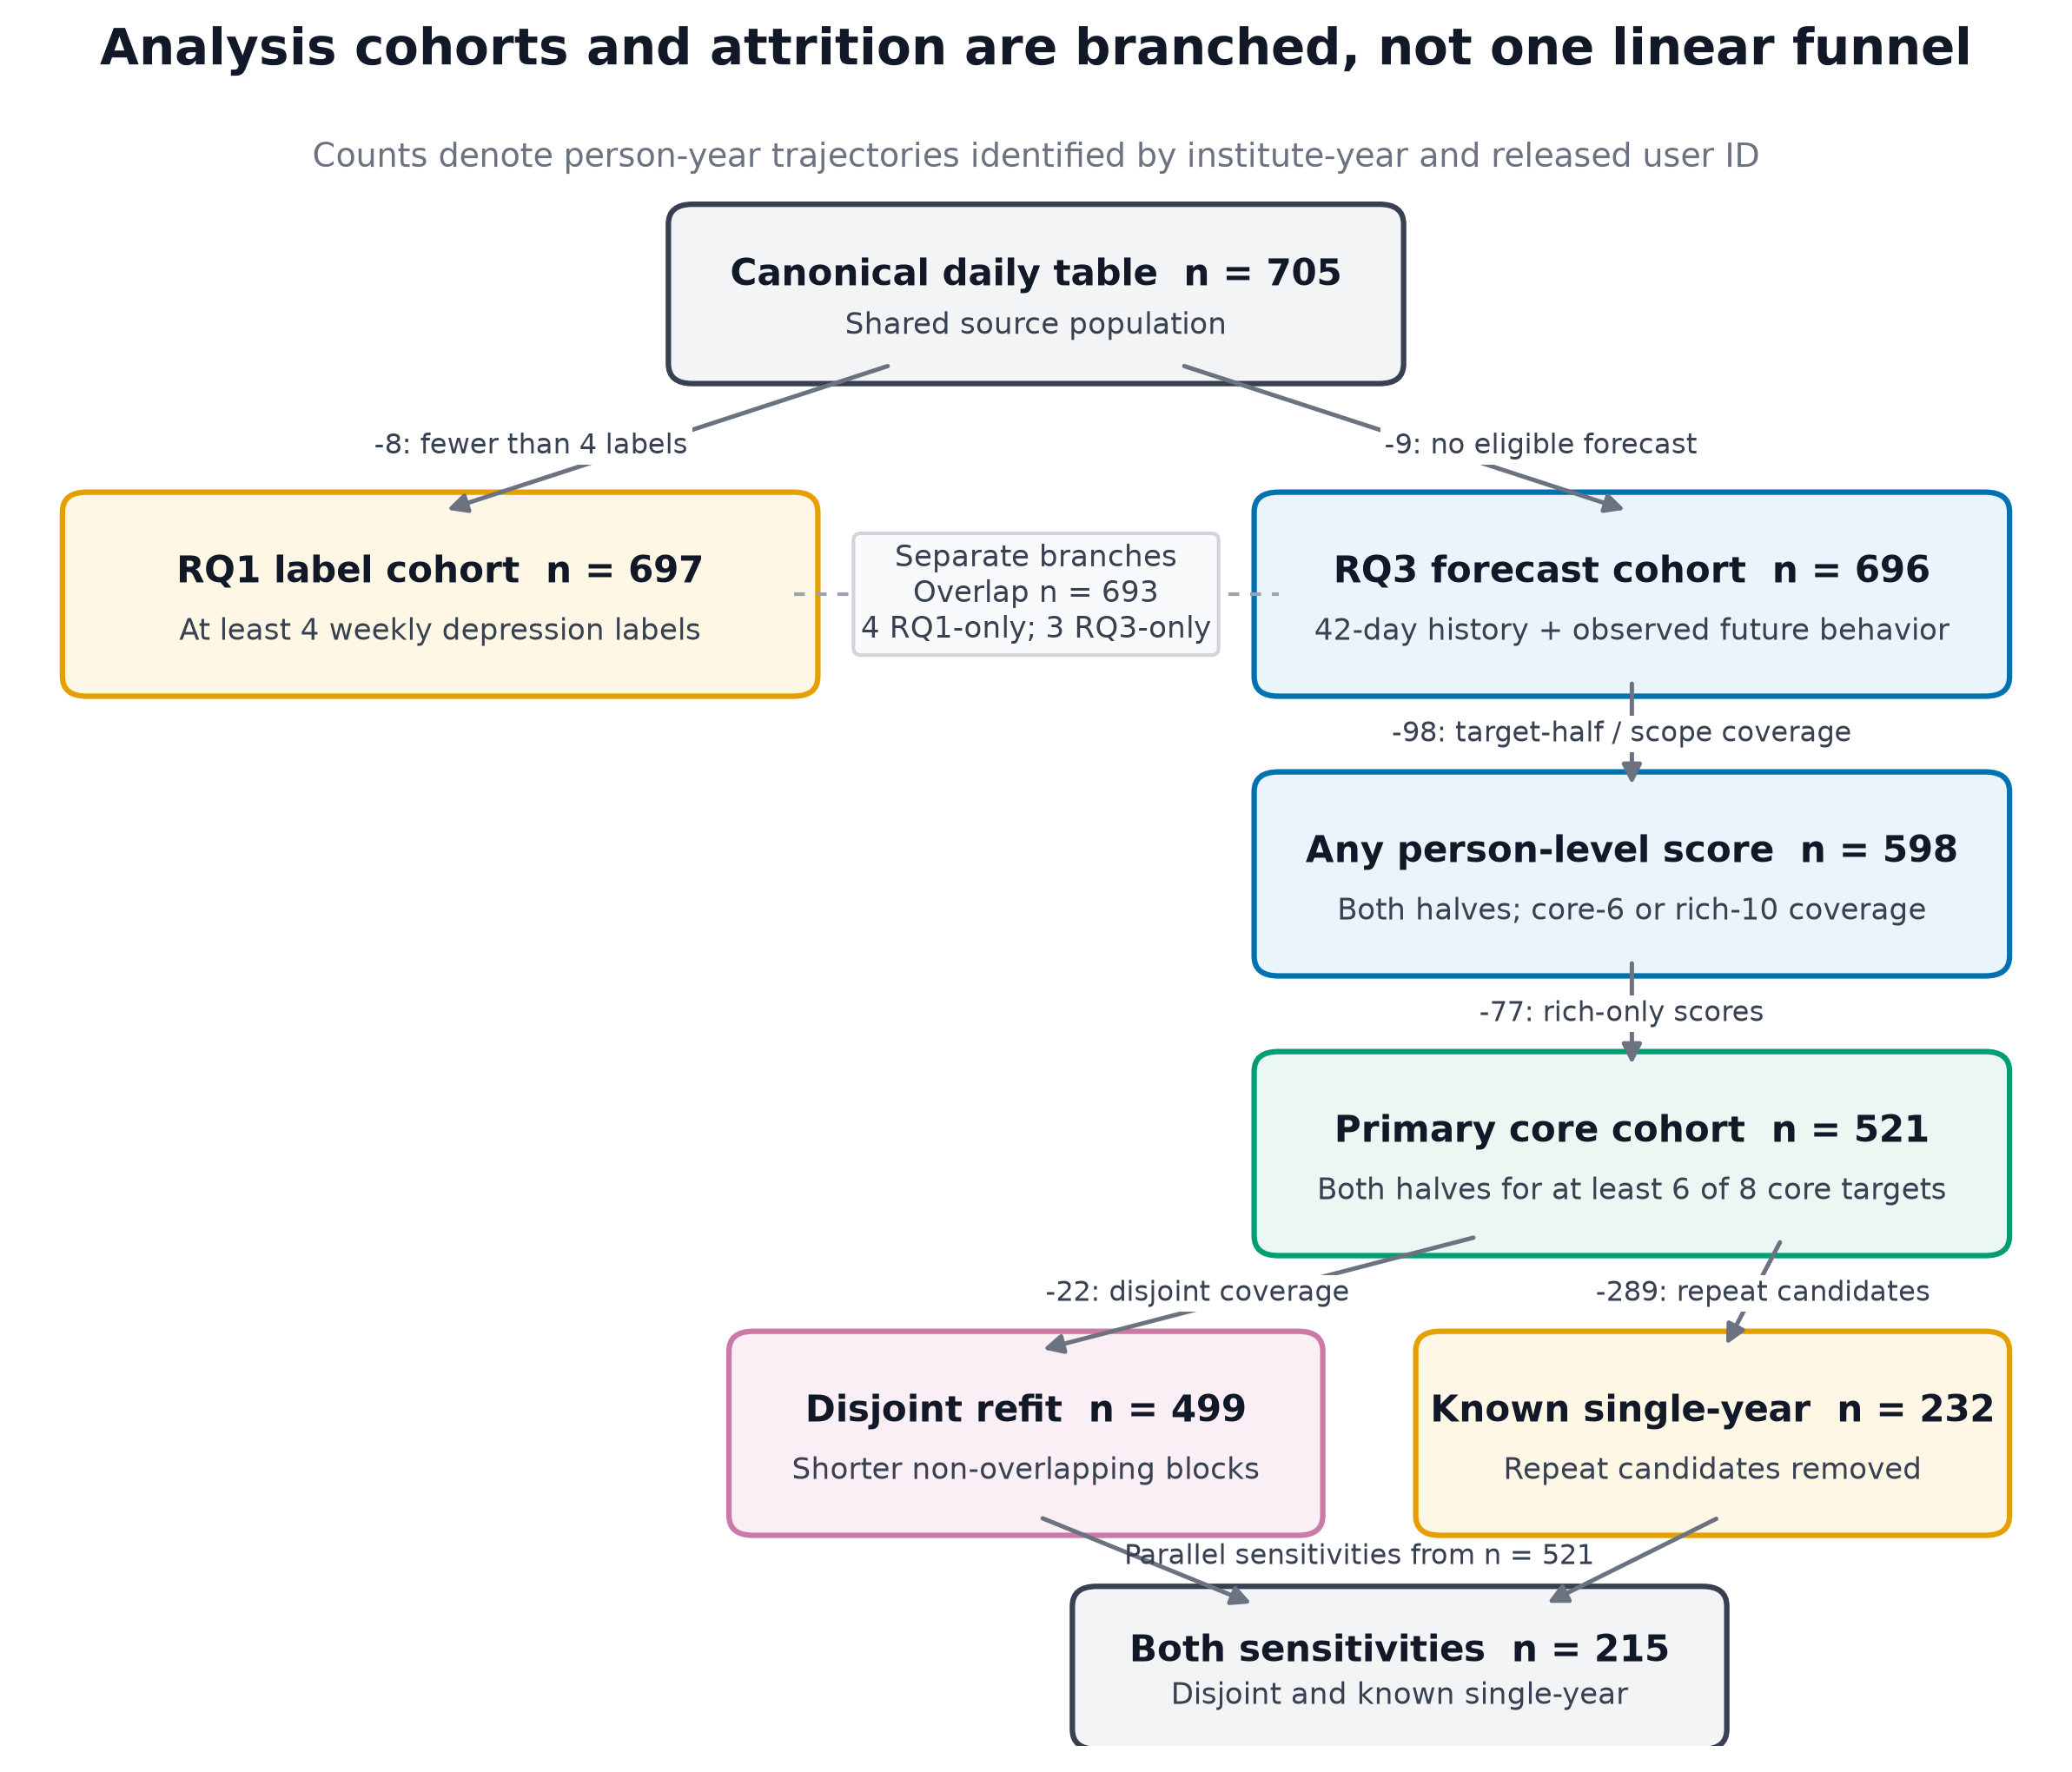
\includegraphics[width=\textwidth]{agent2_sample_attrition_flow.png}
\caption[Analysis-cohort flow and sensitivity branches]{Analysis-cohort flow. RQ1
and RQ3 apply different eligibility rules and overlap on 693 trajectories; neither
is nested in the other. Within RQ3, 521 trajectories form the primary core cohort.
Disjoint refitting ($n=499$) and conservative removal of repeat candidates ($n=232$)
are parallel sensitivities; their intersection contains 215 trajectories.}
\label{fig:sample-attrition}
\end{figure}

\section{Behavioral and psychological variables}

The direct behavior forecast attempted 16 targets derived from released aggregate
features. They covered screen interaction, physical activity, sleep, mobility,
communication, Bluetooth, and Wi-Fi. Continuous targets were modeled on a
$\log(1+y)$ scale. Binary targets were defined relative to the training-set median.

The core construct analysis used eight relatively common targets: screen-unlock
count, screen-unlock duration, steps, active duration, sedentary duration, sleep
duration, time in bed, and sleep efficiency. A 16-target rich-profile sensitivity
was used only as a robustness check.

The psychological audit combined ten repeated outcome columns covering depression,
anxiety, stress, and affect. There were 45 possible pairwise comparisons. Twenty-nine
pairs had finite correlation estimates; the remaining pairs had no or insufficient
same-day overlap. Several columns are derived or closely related representations,
including PHQ-4 variants. The results therefore quantify empirical overlap in the
released analysis table, not ten independent diagnostic instruments.

\subsection{Released depression-screening target}
\label{sec:dep-target}

RQ1 used the released binary column \texttt{dep} from
\texttt{SurveyData/dep\_weekly.csv} without redefining it. This is a screening proxy,
not a clinical diagnosis, and its construction is not identical across cohorts
\citep{xu2022globem,xu2023globemphysionet}. In institute-years 2--4, weekly EMA
observations were positive when the PHQ-4 total score exceeded 2, the release's
threshold for at least mild symptoms. Institute-year 1 did not administer PHQ-4;
the dataset authors instead transferred a depth-2 decision rule learned in year 2
from the PANAS-style ``depressed'' and ``nervous'' items. That rule assigned a
negative label only when depressed was below 2 and nervous was below 3 on their
1--5 scales. The released weekly file also merges the end-term BDI-II screening
observation, whose positive threshold is greater than 13.

Consequently, \texttt{dep} is a cohort-dependent composite of weekly EMA screening
and an end-term screening observation. The present analysis evaluates predictability
of that released benchmark label; it does not re-estimate the instruments, harmonize
their measurement properties, or infer diagnosed depression. In the frozen 65/35
within-trajectory split, 2,367 of 5,213 training rows were positive (45.4\%) and
1,395 of 2,927 test rows were positive (47.7\%).

\section{Preprocessing and missing data}

The analysis used released daily aggregates rather than raw sensor streams. Each
experiment applied its own minimum-history and coverage requirements. Missing data
were not treated as proof of behavior or state. Coverage variables were included in
selected controls, and the follow-up personalization audit used count-only
eligibility checks before any outcomes were analyzed.

The behavior forecast used calendar features, yesterday's outcome, rolling 7-, 14-,
and 42-day summaries, and partial-day features where applicable. Features were
constructed using information available before the prediction target. The target
horizons were tomorrow and the following seven-day mean.

\section{Cross-year identity boundary}

Pinned overlap metadata identified 378 repeat-candidate trajectory keys. Of the 521
core trajectories, 289 were candidates and 232 were known single-year records. The
release did not expose a complete cross-year person identifier, precluding a
person-cluster bootstrap. A conservative sensitivity excluded every repeat candidate;
accordingly, longitudinal claims use the units ``within trajectory'' and
``person-year profile,'' not cross-year person-level stability.

\section{Privacy and data access}

The primary project is a secondary analysis of a de-identified research release.
Recruitment, consent, and institutional-review procedures are described in the
GLOBEM publication \citep{xu2022globem}. This report does not claim a new ethics
approval. No raw GLOBEM data or participant-level follow-up tables are copied into
the report folder or submission repository. The supplementary pilot is
self-observation by the author and includes no third-party participant. Its raw
session logs and exact app identities remain private; only aggregate counts, metrics,
contracts, and de-identified displays are used in the report package.

Quantitative claims and figures trace to machine-readable CSV or JSON outputs through
\path{CLAIM_SOURCE_MAP.md}. Figures are regenerated by \path{make_figures.py} from
aggregate outputs, and the report package contains no restricted participant-level
input data.

\chapter{Project Method}
\label{ch:method}

\section{Staged experimental design}

The project proceeded in seven stages:

\begin{enumerate}
  \item establish passive-sensing and history baselines;
  \item audit psychological labels against prior-label history and construct
  overlap;
  \item forecast direct behavior prospectively;
  \item define and test scalar and profile measures of forecast performance;
  \item run construct, model-refitting, mechanism, and typology controls;
  \item freeze a separate personalization design and stop it if feasibility failed;
  and
  \item instrument and audit a separate single-user Android decision pilot.
\end{enumerate}

Early results motivated later construct checks, which attributed most scalar
forecastability stability to behavioral variance and changed the scientific
interpretation of that score.

\section{Chronological evaluation}

For the main behavior forecast, each trajectory was split chronologically. The
earlier 65\% supplied the original training period, and the later 35\% supplied
prospective evaluation rows. No future target values were used to construct history
features for an earlier prediction.

The psychological-label control also used a within-user temporal split. Its
prior-label feature used expanding prior labels in training and the user's
training-period label rate for test rows. A training global rate was used when a
user-specific rate was unavailable.

\section{Psychological-label baselines}

Random-forest depression classifiers compared five feature sets:

\begin{enumerate}
  \item current-day all-day passive features;
  \item 7/14-day passive history;
  \item prior same-person depression-label rate only;
  \item current-day passive features plus prior-label rate; and
  \item passive history plus prior-label rate.
\end{enumerate}

The primary metric was held-out AUROC. For the two combined-versus-label-only
contrasts, uncertainty was estimated by a paired 10,000-draw bootstrap over 697
released person-year trajectories; every sampled trajectory contributed all of its
test rows. A 95\% interval containing zero was defined as no detectable increment.

A within-person ranking test then retained only test trajectories containing both
depression-label classes. AUROC was computed inside each trajectory and averaged
equally across trajectories; a trajectory-constant predictor therefore scores 0.5
and cannot benefit from between-person prevalence. The primary rule required the
history-plus-prior mean AUROC to reach 0.55 with a trajectory-bootstrap interval
entirely above 0.5. A post-hoc design diagnostic conditioned on the observed positive
and negative row counts and simulated common binormal ranking effects. It quantified
the sensitivity of the aggregate mean, while the short trajectories remained
insufficient for person-specific performance estimates. A separate robustness grid
crossed three temporal test fractions with three random-forest initializations.

For construct overlap, all possible same-day pairs among ten repeated psychological
columns were examined. The primary sensitivity excluded comparisons among four
PHQ-derived representations and required at least 100 same-day observations per
pair. Ridge models then predicted each target using its own prior, other constructs'
priors, or both. These models quantify overlap and persistence. They are not
passive-sensing models.

\section{Prospective behavior forecasting}

Six model specifications were evaluated for each target, horizon, and issue time:
calendar only; recent history; a 42-day fingerprint; partial-day behavior; history
plus fingerprint; and history plus fingerprint plus partial-day behavior. Continuous
targets used ridge regression. Binary high/low targets used logistic regression.

The models were pooled across eligible training rows. They were not fitted separately
for each person-year trajectory. Held-out $R^2$ and AUROC were summarized across 16
heterogeneous targets using both means and median/IQR. Neither summary represents
one task, so per-target values are retained in the appendix.

\section{Model implementation}

\Cref{tab:model-config} records the settings needed to interpret the headline
models. Settings are reported only when they are explicit in the runner or its
configuration. The project configuration does not pin the scikit-learn version;
therefore a setting left to a library default is identified rather than silently
treated as an immutable parameter.

\begin{table}[H]
\centering
\footnotesize
\caption[Headline model implementation]{Headline model implementation and explicit
configuration. All scaling and imputation statistics were fitted on training rows.
Exact runners and checked outputs are listed in \cref{app:work-packages}.}
\label{tab:model-config}
\begin{tabularx}{\textwidth}{@{}L{0.20\textwidth}L{0.22\textwidth}Y@{}}
\toprule
Stage & Estimator & Essential settings \\
\midrule
Depression-label audit & Random-forest classifier & Median imputation; 300 trees;
minimum leaf size 5; balanced class weights; all CPU cores; no feature scaling. \\
Construct-prior audit & Closed-form ridge regression & Training-median imputation
and standardization; $\alpha=10$; unpenalized intercept; 65/35 within-trajectory
temporal split. \\
Behavior forecast & Ridge and logistic regression & Training-median imputation and
standardization. Regression used ridge with $\alpha=1$. Classification used balanced
logistic regression with \texttt{liblinear}, 1,000 iterations, and the non-overridden
scikit-learn defaults L2 penalty and $C=1$. \\
Forecastability refits & Custom ridge regression & Median imputation,
standardization, $\alpha=1$, fixed/expanding/disjoint temporal regimes, 1,000
bootstrap draws, and 10,000 headline permutations. \\
Mechanism follow-up & Custom ridge regression & Same estimator with $\alpha=1$,
1,000 bootstrap draws, and 10,000 headline permutations. \\
Typology follow-up & Spherical $k$-means & $k=2,\ldots,5$; 30 initializations; 100
iterations per fold; leave-one-cohort-out assignment; 500 permutations. \\
\bottomrule
\end{tabularx}
\end{table}

\section{Initial and corrected operationalizations of forecastability}

The initial analysis operationalized forecastability for trajectory $u$, target
$k$, and held-out half $h$ as global-SD-normalized negative mean absolute error:

\begin{equation}
F_{ukh}=-\frac{1}{\sigma_k}\frac{1}{|I_{ukh}|}
\sum_{i\in I_{ukh}}\left|y_i-\widehat{y}^{\,\mathrm{hist}}_i\right|,
\label{eq:forecastability}
\end{equation}

where $\sigma_k$ is the target's global log-scale standard deviation. Higher values
mean lower absolute error. This estimator was reproducible enough to support the
initial analysis, but it was mis-specified for the intended person-relative
construct. Its denominator is constant across trajectories within a target: it
neither adjusts for person-level outcome scale nor asks whether history improves on
a relevant comparator. Equation~\ref{eq:forecastability} is retained as the audited
historical operationalization, not as a validated forecastability phenotype.

The corrected comparator-relative operationalization was

\begin{equation}
S_{ukh}=1-\frac{\mathrm{MAE}^{\mathrm{hist}}_{ukh}}
{\mathrm{MAE}^{\mathrm{calendar}}_{ukh}}.
\label{eq:skill}
\end{equation}

Both errors are evaluated for the same trajectory, target, and held-out half. $S$
asks how much the pooled history model improves on the pooled calendar model in that
context. It corrects the absence of a comparator in
Equation~\ref{eq:forecastability}, but remains sensitive to the calendar model,
denominator error, marginal entropy, and population-average coefficients. It is not
a measure of separately fitted personal-model skill.

Target-half measures were standardized within target. Equal-weight averages formed
scalar degree scores. Cross-target vectors formed continuous domain profiles.
Profile similarity used cosine similarity.

\section{Decision rules and provenance}

The project record specified three decision rules before the corresponding full
inferential run. Because that record lacks an independent prospective timestamp,
the rules organize the internal analysis but are not presented as preregistration.

\begin{itemize}
  \item \textbf{H1 scalar stability:} early/late Pearson $r\geq0.30$ with a
  trajectory-bootstrap 95\% confidence interval above zero.
  \item \textbf{H2 profile stability:} same-trajectory early/late cosine similarity
  exceeds institute-year-matched cross-trajectory similarity by $\Delta\geq0.10$
  with permutation $p<0.05$.
  \item \textbf{H3 trait association:} corrected association with selected traits
  has $|r|\geq0.10$ and max-statistic permutation $p<0.05$.
\end{itemize}

The numeric thresholds are project-specific rather than universal psychometric
standards. The H1 rule was statistically suboptimal: it applied the practical
threshold to the point estimate while testing the confidence bound only against
zero. The historical decision is retained for transparency, but an interval spanning
0.30 is inconclusive about whether the population effect meets that value. A future
confirmatory analysis should test uncertainty against the practical threshold.

\section{Model-artifact and construct controls}

Three temporal model regimes tested whether shared fitted coefficients produced
apparent stability:

\begin{description}
  \item[Fixed.] The original pooled model scored both test halves.
  \item[Expanding refit.] The model was refitted after the first test half before
  scoring the final half.
  \item[Disjoint refit.] Separate models were trained on disjoint early and late
  windows and evaluated on later windows.
\end{description}

Construct overlap was tested against observed target standard deviation and
normalized marginal quintile entropy. A stronger sensitivity estimated these moments
from the corresponding training block to avoid sharing the same held-out observations
with MAE. Full-trajectory sequence controls added first-order conditional entropy,
weekday-conditional entropy, and a Lempel--Ziv proxy. These are descriptive controls,
not theoretical entropy-rate ceilings.

\section{Uncertainty and multiplicity}

RQ1 incremental uncertainty used a paired 10,000-draw trajectory-clustered
bootstrap. The within-person test also used 10,000 trajectory bootstrap draws after
restricting evaluation to trajectories with both label classes. These resampling
procedures preserve repeated observations inside released person-year trajectories;
they do not reconstruct unavailable cross-year identities.

Split-half correlations used 1,000 trajectory bootstrap samples. Matched profile
contrasts used within-cohort permutations with finite-sample correction. Headline
residual profiles used 10,000 permutations and are reported as $p<0.001$ when they
reached the resampling resolution. Secondary feature-family and original
profile tests used 500 permutations; their resolution floor is $p=0.002$.

The H3 trait test used corrected inference. A later Fisher-$z$ approximation estimated
an 80\% minimum detectable absolute correlation of about 0.17 under a conservative
28-test Bonferroni approximation. This was larger than the 0.10 effect gate, so a
failed H3 is treated as inconclusive rather than evidence of independence.

Feature-family decomposition and mechanism tables are explicitly post-hoc. Their
individual permutation probabilities were not adjusted to support family-wise
confirmatory inference; the report therefore treats them as robustness leads rather
than independent discoveries.

\section{Mechanism and typology follow-up}

The post-hoc mechanism audit separated calendar terms, yesterday's outcome,
7/14-day rolling means, a 42-day mean/standard-deviation fingerprint, all own-domain
history, and recent histories from the other seven core domains. A feature family
was considered an exploratory lead only if its adjusted scalar and profile gates
held in all three model regimes.

Cross-domain coupling had an additional performance requirement: aggregate held-out
MAE had to improve, and at least six of eight targets had to improve. Discrete
typology used spherical $k$-means for $k=2$ through $5$. Clusters were trained on
three cohorts and tested without refitting in the fourth. The typology gate required
median adjusted Rand index (ARI) above 0.20, sufficient prevalence, and successful
assignment stability in at least three held-out cohorts, including under disjoint
refitting. With only four cohorts, this is a coarse four-trial stress test rather
than strong external validation.

\section{Personalization feasibility gate}

A separate contract proposed a leave-one-institute-year-out personalization study.
Phase A was outcome-blind and count-only. It required at least 30 eligible
person-targets in every institute-year and at least 160 in total for selected target
families. The contract required the study to stop before modeling if no allowed
branch passed. This prevented a data-dependent relaxation after seeing prediction
outcomes.

\section{Implemented work packages}
\label{sec:implementation}

\Cref{tab:work-packages-main} summarizes the project sequence. On the same 196
RAPIDS history features and outer splits, the hygienically validated MLP achieved
AUROC 0.619 within user and 0.559 on held-out users, compared with 0.691 and 0.577
for the random forest. A legacy LSTM on a different raw 14-day sequence reached
0.622 and 0.553; because its input and retained validation evidence differ, it is
context rather than a matched comparison. Full model metrics and validation scope
are reported in \cref{app:neural-diagnostics}. Subsequent analyses therefore focused
on target validity and strong non-sensor comparators rather than increasing neural
capacity.

\begin{table}[H]
\centering
\small
\caption[Implemented work packages]{Implemented work packages and decisive outcomes. Detailed runner, contract, and
output paths are retained in \cref{app:work-packages} and the repository source map.}
\label{tab:work-packages-main}
\begin{tabularx}{\textwidth}{@{}L{0.09\textwidth}L{0.23\textwidth}Y L{0.14\textwidth}@{}}
\toprule
WP & Work performed & Decisive outcome & Status \\
\midrule
1 & Baseline and model exploration & The matched-input MLP remained below the
history RF; a differently specified legacy LSTM was also lower. &
Mixed/null \\
2 & Label-history and construct audit & No detectable passive increment in clustered
or within-person tests; cross-family outcomes overlapped. & Primary boundary \\
3 & Prospective behavior forecast & Direct behaviors were forecastable across 16
targets, with most performance supplied by simple same-channel history. & \passed \\
4 & Forecastability construct audit & Raw stability survived refitting but was
largely variability; adjusted point estimate $r=0.230<0.30$ while its CI crossed
the gate. & \failed \\
5 & Post-hoc structure and typology & Continuous profile survived tested controls;
cross-domain increment and discrete typology failed. & \exploratory/mixed \\
6 & Personalization feasibility & Outcome-blind eligibility left no allowed
multi-family branch; no model was fitted. & \stopped \\
7 & Android self-instrumentation pilot & Custom logger, provenance freeze, and
chronological policy audit on the author's own data; observed policies were worse
than no action. & \exploratory/\failed \\
\bottomrule
\end{tabularx}
\end{table}

The original forecastability run passed its raw scalar and profile criteria, but the
later construct audit attributed most scalar stability to behavioral variance. The
separate personalization audit stopped before outcomes were examined and did not
estimate a prediction effect.

\chapter{Results}
\label{ch:results}

\section{RQ1: psychological-label validity boundary}

\subsection{Prior labels exceeded passive models}

The target was the released cohort-dependent depression-screening proxy defined in
\cref{sec:dep-target}. The chronological split contained 5,213 training observations
(2,367 positive; 45.4\%) and 2,927 test observations (1,395 positive; 47.7\%).
Current-day passive features achieved AUROC 0.579. Passive history achieved 0.691.
The prior same-person label rate alone achieved 0.844. Current-day features plus the
label rate achieved 0.840, and passive history plus the label rate achieved 0.841.
Both combined models were lower than the label-only baseline
(\cref{fig:validity-auroc,tab:label-results}). There was no positive increment beyond
label history at the point-estimate level.

\begin{figure}[H]
\centering
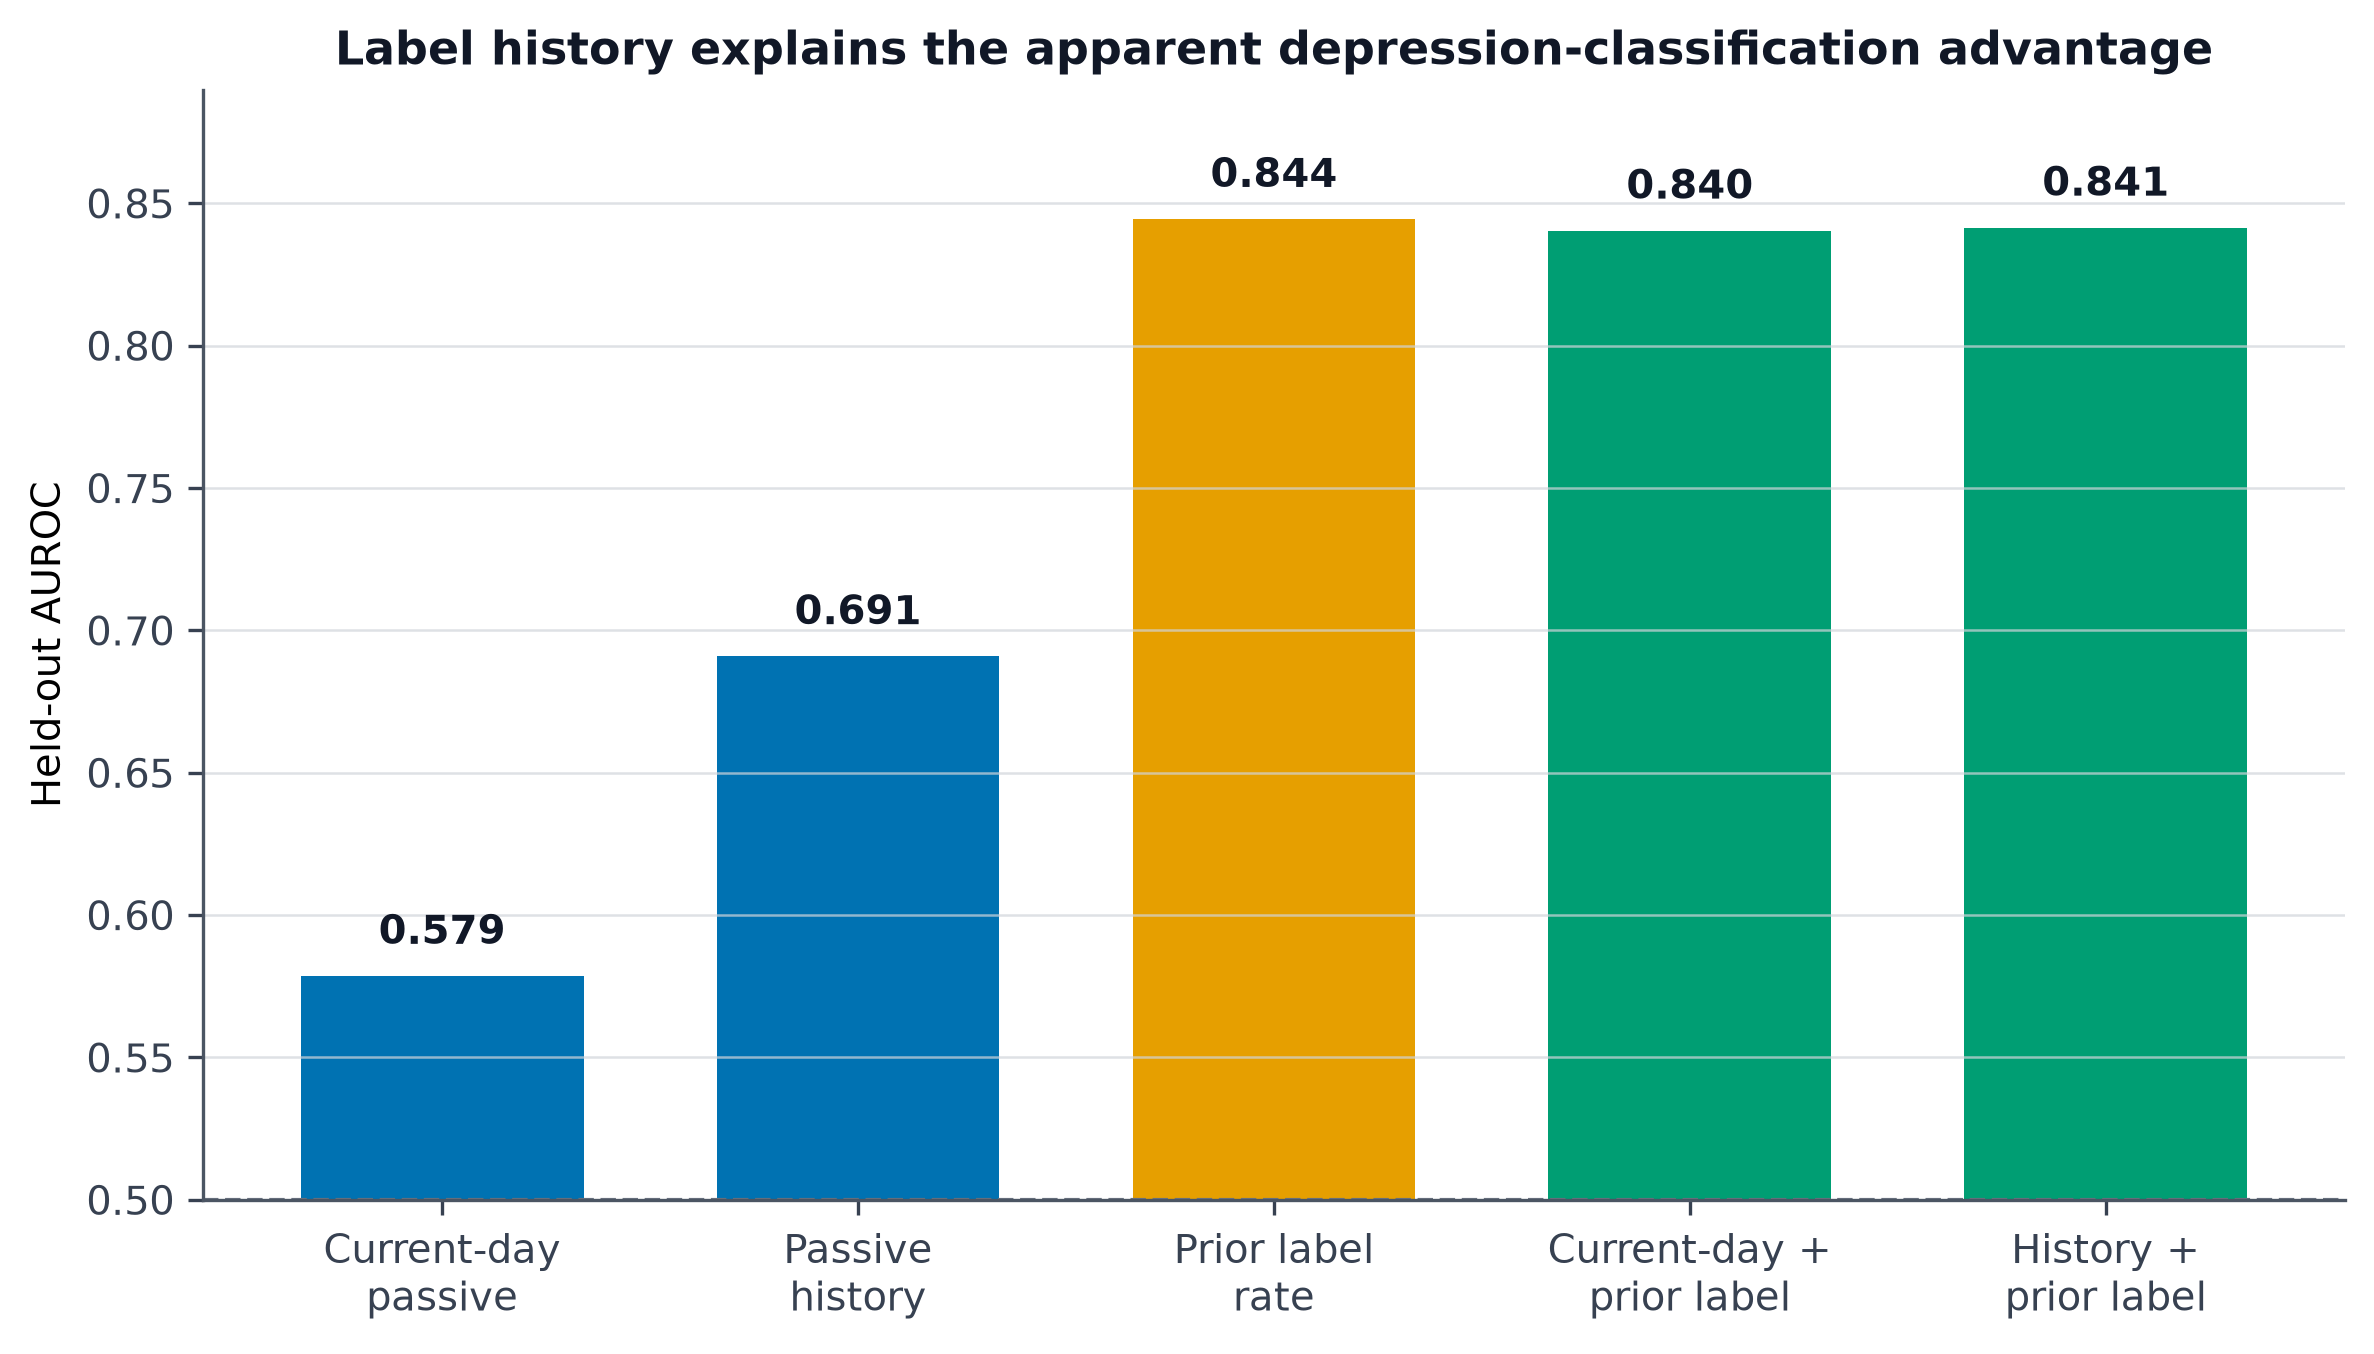
\includegraphics[width=\textwidth]{validity_boundary_auroc.png}
\caption[Depression-screening-label AUROC with and without label history]{Held-out AUROC for the released depression-screening proxy in the chronological
label-baseline control. The analysis used 5,213 training rows (45.4\% positive) and
2,927 test rows (47.7\% positive). The label-only baseline scored 0.844. Current-day plus label and history plus
label scored 0.840 and 0.841, respectively. Their clustered increment intervals
included zero, yielding no detectable increment over label-only. The prior-label
feature is a self-report persistence/prevalence baseline, not a passive sensing
model.}
\label{fig:validity-auroc}
\end{figure}

\begin{table}[H]
\centering
\caption[Depression-screening-label classification results]{Classification of the
released depression-screening proxy. The 5,213/2,927 chronological train/test rows
were 45.4\%/47.7\% positive. Differences were calculated from unrounded outputs and
are shown to three decimals.}
\label{tab:label-results}
\begin{tabularx}{\textwidth}{@{}Y S[table-format=1.3]
S[table-format=-1.3] L{0.24\textwidth}@{}}
\toprule
Feature set & {AUROC} & {\makecell{Difference vs.\\label-only}} & Interpretation \\
\midrule
Current-day passive & 0.579 & -0.266 & Passive-only \\
Passive history & 0.691 & -0.154 & Passive-only \\
Prior label rate only & 0.844 & 0.000 & Strongest baseline \\
Current-day passive + prior label & 0.840 & -0.004 & No positive increment \\
Passive history + prior label & 0.841 & -0.003 & No positive increment \\
\bottomrule
\end{tabularx}
\end{table}

The published GLOBEM benchmark provides context but not a like-for-like
reproduction. In the authors' ``Users Past/Future within One Dataset'' setup, the
first 80\% of each user's observations trained a model and the final 20\% tested it
within each dataset \citep{xu2022globem}. Its headline
$0.691\mathbin{\pm}0.018$ for Xu et al.-I is balanced accuracy, whereas 0.691 here
is pooled ROC AUROC; the corresponding published mean ROC AUC was 0.737. On matched
metric names, the present passive-history model was descriptively lower (balanced
accuracy 0.642 versus 0.691; ROC AUROC 0.691 versus 0.737). The evaluations are not
exchangeable: this study used a pooled 65/35 split, 7/14-day screen, step, and sleep
history, and a fixed random forest, whereas Xu et al.-I used separate per-dataset
80/20 splits, a broader multi-epoch feature pipeline, association-rule filtering,
and AdaBoost. The comparison anchors model strength without claiming a failed
reproduction.

Paired trajectory-clustered inference supported the same, narrower conclusion
(\cref{tab:rq1-clustered}). The current-day contrast was $-0.004$ with 95\%
interval $[-0.013,0.005]$; the history contrast was $-0.003$ with interval
$[-0.013,0.007]$. Both intervals contain zero, so the result is no detectable
increment, not proof that the true effects are exactly zero or negative.

\begin{table}[H]
\centering
\small
\caption[RQ1 trajectory-clustered inference]{Paired held-out AUROC differences
versus the prior-label-rate-only baseline. Intervals use 10,000 bootstrap resamples
of 697 released person-year trajectories and retain all rows within each sampled
trajectory.}
\label{tab:rq1-clustered}
\begin{tabularx}{\textwidth}{@{}L{0.34\textwidth}C{0.12\textwidth}
C{0.22\textwidth}Y@{}}
\toprule
Combined model & $\Delta$ AUROC & 95\% clustered CI & Decision \\
\midrule
Current-day passive + prior label & -0.004 & $[-0.013,0.005]$ & No detectable increment \\
Passive history + prior label & -0.003 & $[-0.013,0.007]$ & No detectable increment \\
\bottomrule
\end{tabularx}
\end{table}

The within-person analysis retained 295 trajectories and 1,295 test rows with both
label classes. The primary history-plus-prior model achieved an equal-weight mean
within-trajectory AUROC of 0.514 (95\% CI $[0.474,0.556]$); the pair-weighted value
was 0.522. Current-day-plus-prior reached 0.534 (95\% CI $[0.494,0.575]$).

Individual trajectories were sparse: the median was four test rows (IQR 4--5) and
three positive-negative pairs (IQR 3--4). A post-hoc simulation preserving these
class counts estimated 80\% power for a common AUROC between 0.55 and 0.56, or
between 0.56 and 0.57 for the complete rule that also required a point estimate of
at least 0.55. Thus the aggregate analysis did not detect a moderate shared ranking
effect, but it cannot exclude subtle or heterogeneous effects and cannot estimate
usefulness for an individual user.

The post-hoc split/seed grid reinforced this boundary. Current-day-plus-prior and
history-plus-prior were below prior-only in all nine combinations. Median differences
were $-0.013$ (range $-0.015$ to $-0.004$) and $-0.004$ (range $-0.012$ to
$-0.001$), respectively.

These results apply to the tested GLOBEM cohort, depression target, feature sets, and
model class. Within that scope, passive sensing supplied neither a detectable
aggregate increment over label history nor a detectable moderate shared
within-trajectory ranking effect.

\subsection{Psychological measures overlapped}

The construct audit contained 17,346 rows with at least one psychological measure.
The full released-column summary had 29 finite estimates from 45 possible same-day
pairs and median absolute Pearson correlation 0.663 (IQR 0.532--0.793). That number
mixes distinct constructs with redundant PHQ-derived representations. After
excluding within-PHQ-family comparisons and requiring at least 100 same-day rows,
22 cross-family pairs remained; their median absolute correlation was 0.590 (IQR
0.251--0.722). \Cref{fig:construct-overlap} shows the individual estimates and
missing comparisons.

\begin{figure}[H]
\centering
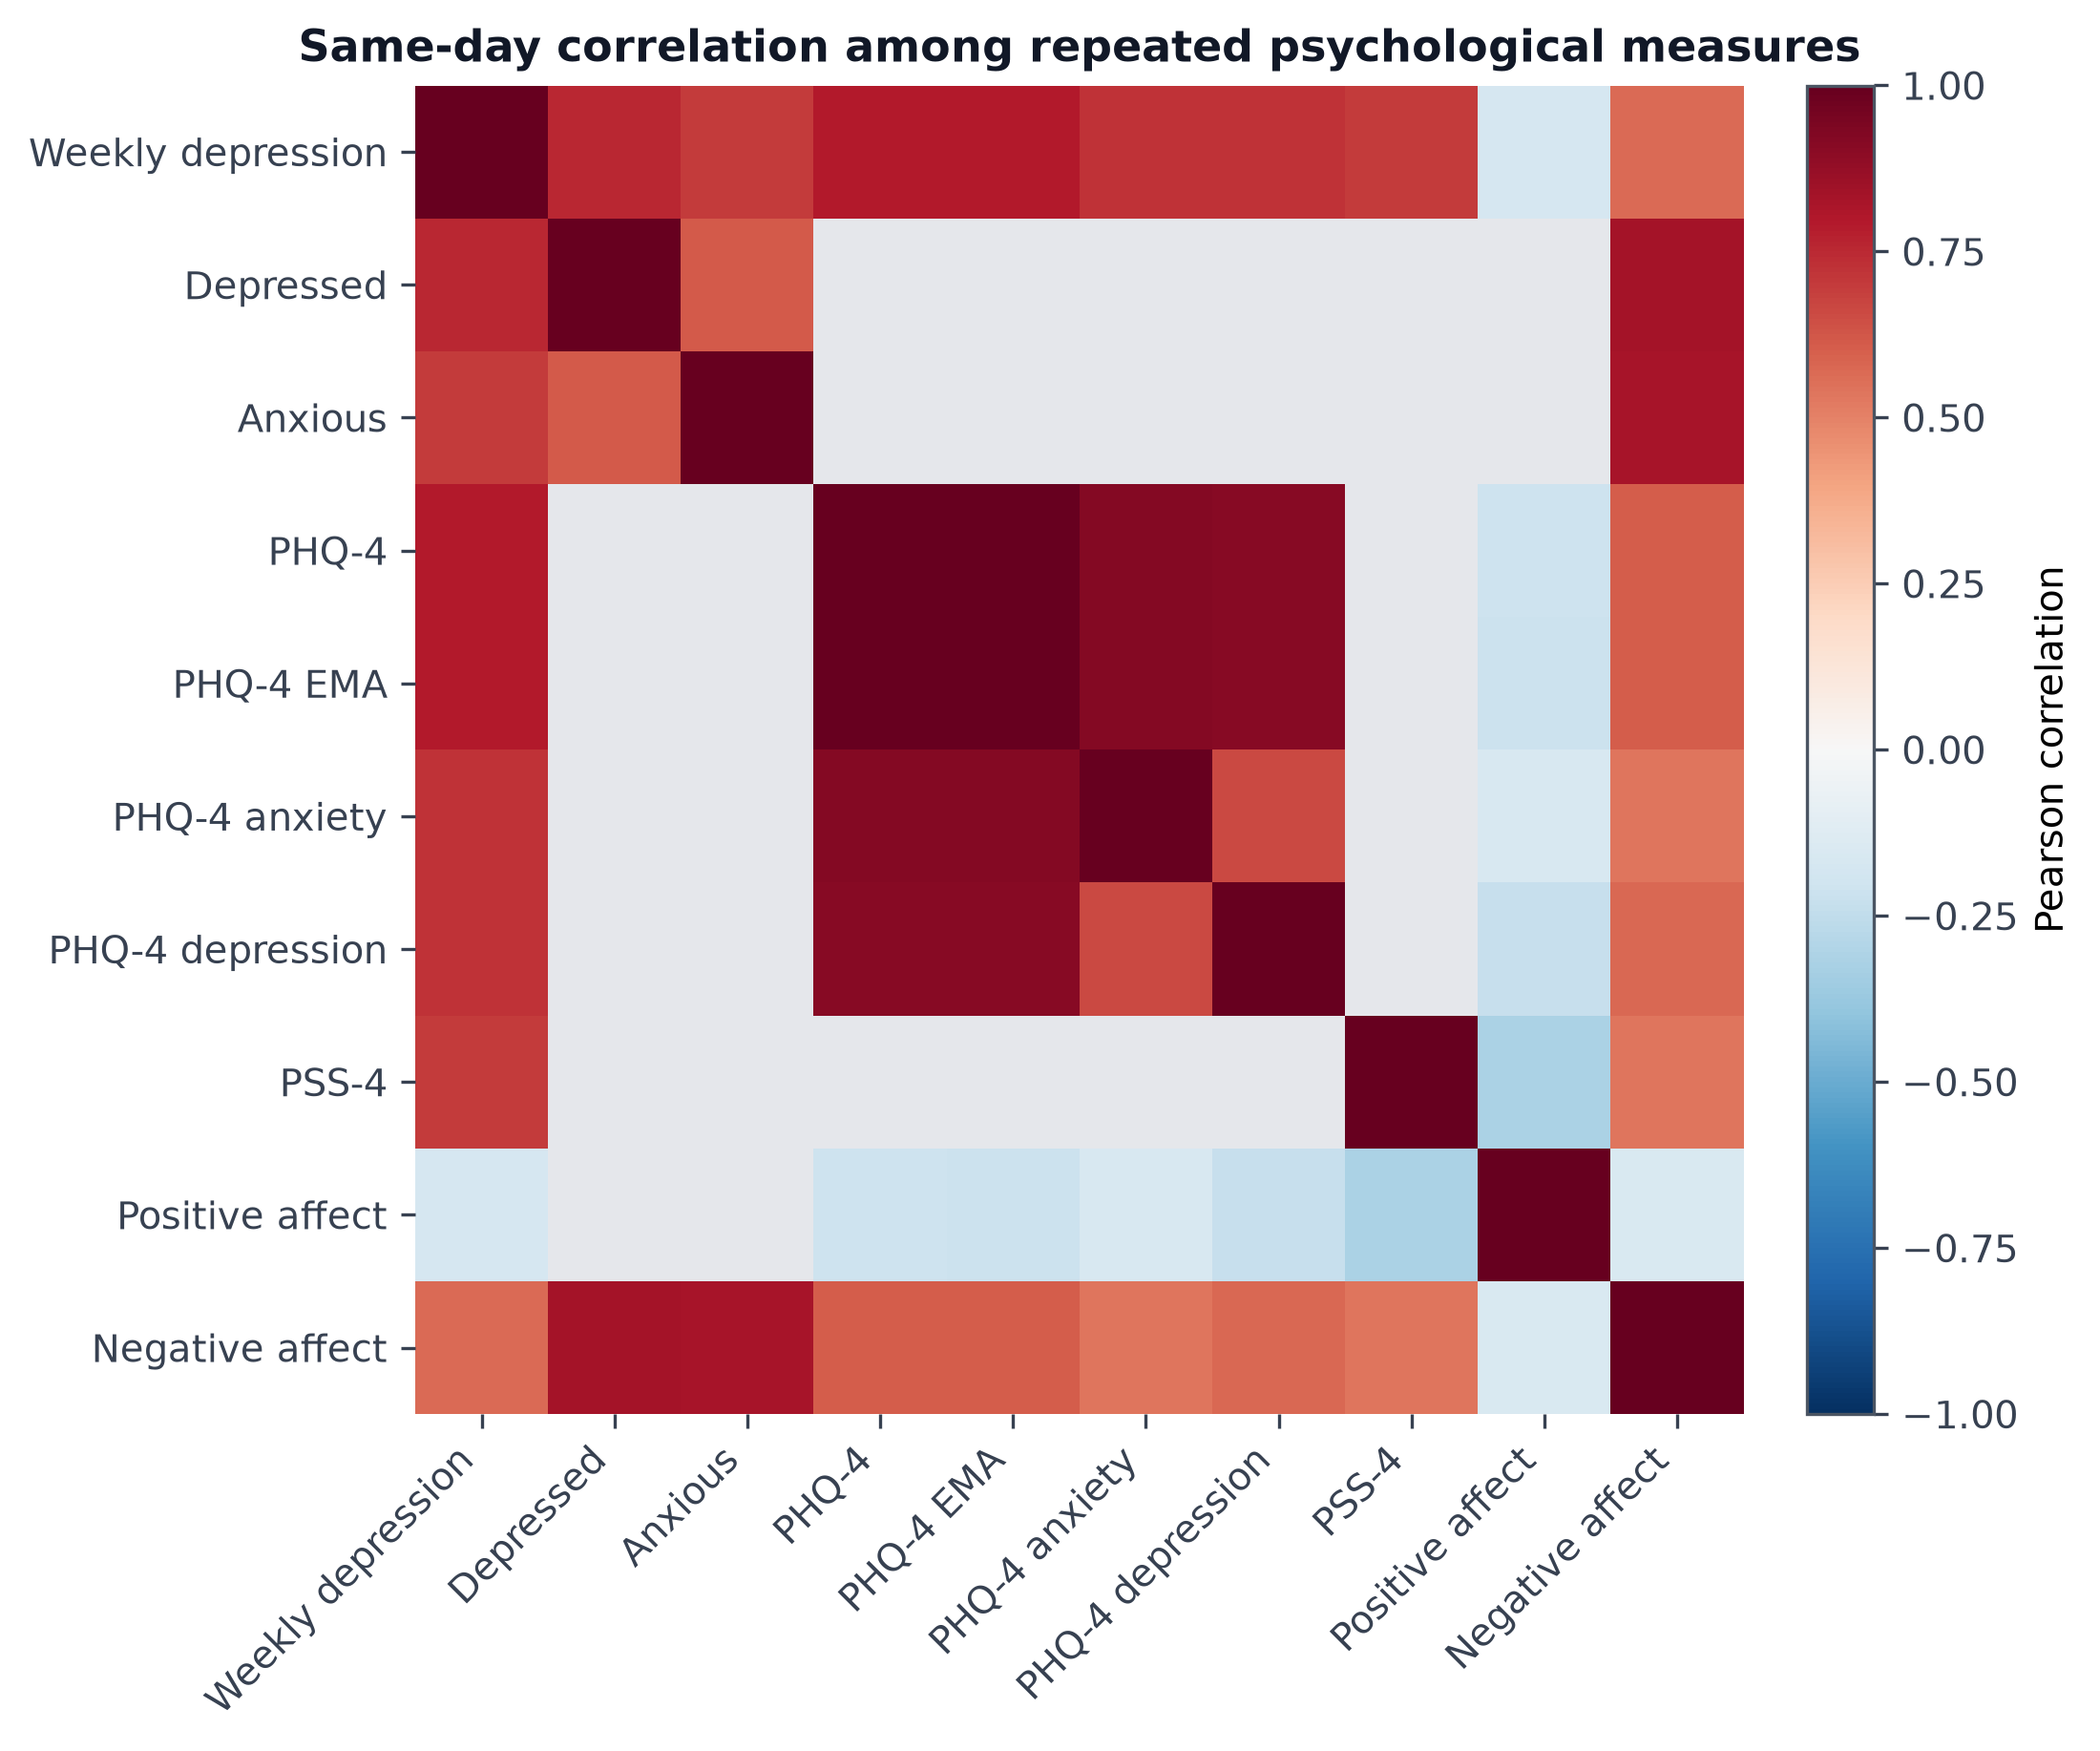
\includegraphics[width=0.92\textwidth]{construct_overlap_heatmap.png}
\caption[Same-day correlation among repeated psychological measures]{Same-day Pearson correlation among ten repeated psychological columns.
Gray cells have no finite estimate because same-day overlap was absent or
insufficient. Across all 29 finite pairs, the mixed median absolute correlation was
0.663. The primary nonredundant sensitivity used 22 cross-family pairs with at least
100 observations and had median 0.590 (IQR 0.251--0.722).}
\label{fig:construct-overlap}
\end{figure}

Mean held-out $R^2$ was 0.479 when each target used its own prior and 0.426 when it
used only other constructs' priors. Adding other priors to the own-prior model
increased mean $R^2$ by 0.044. Other-construct priors approached but did not equal
own-prior prediction on average. No formal equivalence test was performed.

\section{RQ2: directly observed behavior was forecastable}

Across 16 targets, the full evening model achieved median held-out tomorrow
$R^2=0.260$ (IQR 0.225--0.323) and AUROC 0.795 (IQR 0.730--0.830). Means were
0.272 and 0.788. For the following seven-day aggregate, medians were $R^2=0.579$
(IQR 0.408--0.657) and AUROC 0.875 (IQR 0.829--0.920); means were 0.506 and
0.871 (\cref{fig:behavior-performance,tab:behavior-results,tab:rq2-per-target}).
These summaries span heterogeneous tasks and are not the performance of one target.

The baseline hierarchy materially changes the interpretation. Calendar-only models
had mean tomorrow $R^2=-0.007$ and AUROC 0.544. Adding calendar terms, yesterday's
outcome, and 7/14-day means (the recent-history comparator) raised performance to
$R^2=0.244$ and AUROC 0.767. A calendar-plus-42-day mean/standard-deviation baseline
reached 0.252 and 0.777. Combining recent and 42-day history reached 0.259 and 0.782;
the current partial day supplied only the final 0.013 $R^2$ and 0.006 AUROC. The
seven-day horizon followed the same ordering. Thus the supported result is mostly
same-channel behavioral persistence, with small average increments from multiscale
combination and the partial day.

\begin{figure}[H]
\centering
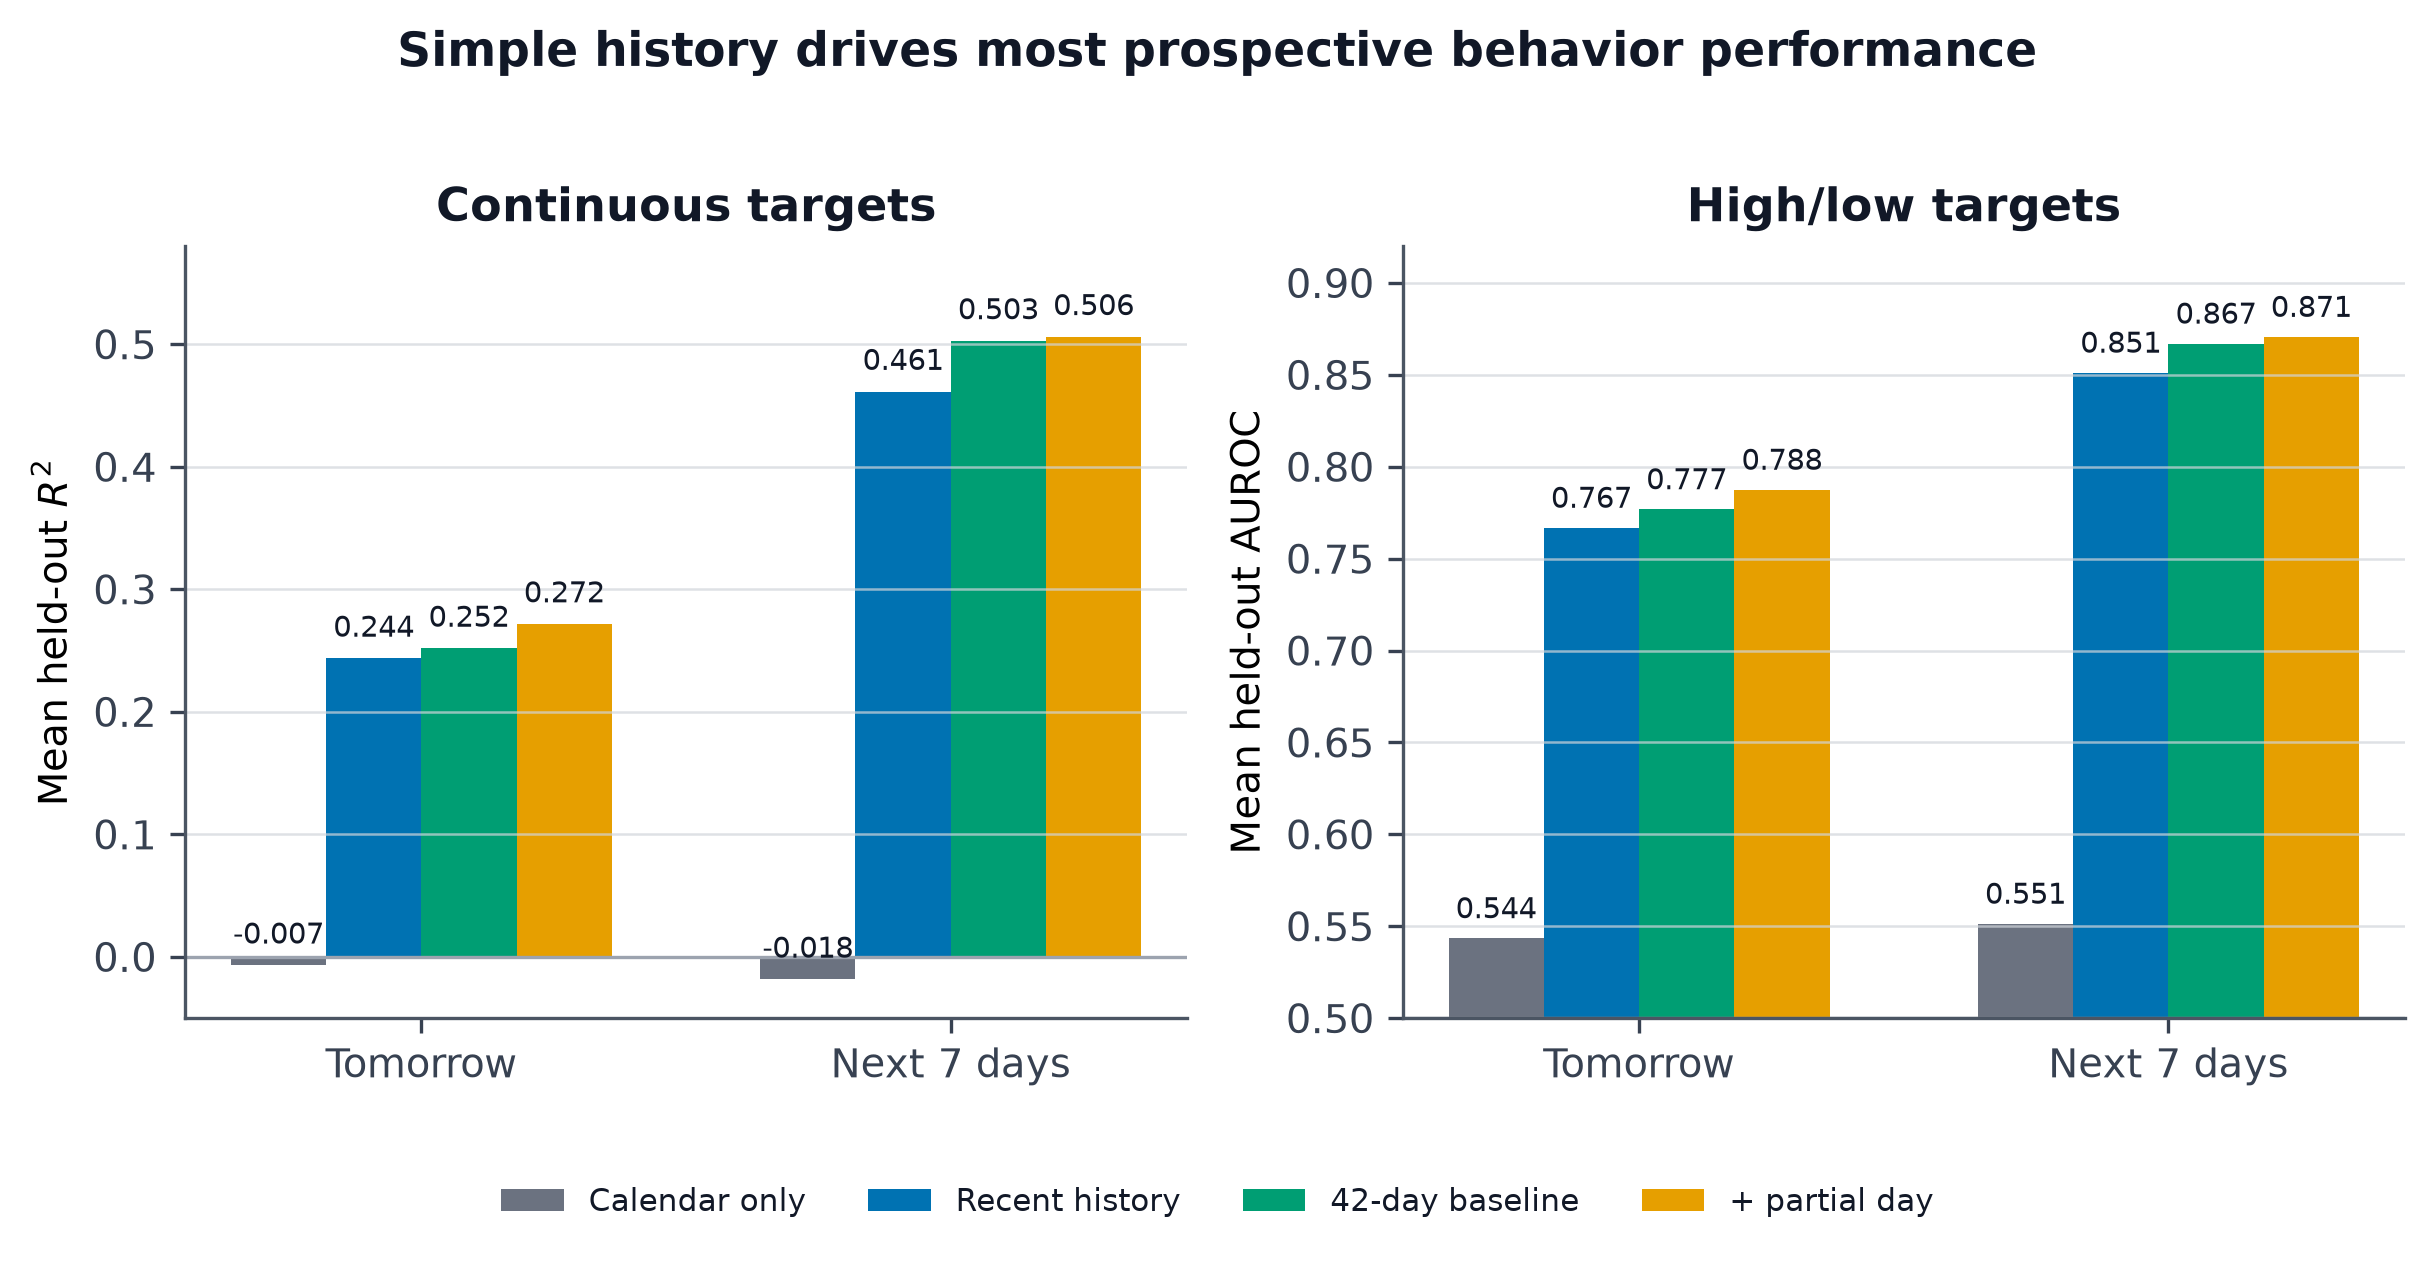
\includegraphics[width=\textwidth]{behavior_forecasting_performance.png}
\caption[Prospective behavior forecasting against simple baselines]{Prospective performance averaged across 16 behavioral targets at the evening issue
time. Calendar-only models are followed by recent history (calendar, yesterday, and
7/14-day means), the 42-day baseline (calendar, 42-day mean and standard deviation),
and the complete history/fingerprint/partial-day model. Continuous targets use
held-out $R^2$; high/low targets use held-out AUROC. No common confidence interval is
available for these heterogeneous target means.}
\label{fig:behavior-performance}
\end{figure}

\begin{table}[H]
\centering
\footnotesize
\setlength{\tabcolsep}{3pt}
\caption[Behavior-forecast baseline hierarchy]{Mean held-out behavior-forecast
performance across 16 targets at the evening issue time. Recent history contains
calendar terms, yesterday, and 7/14-day means. The 42-day baseline contains calendar
terms plus the 42-day mean and standard deviation. Median/IQR and full-model
per-target values are reported in the text and appendix.}
\label{tab:behavior-results}
\begin{tabular}{@{}llSSSSS@{}}
\toprule
Horizon & Metric & {Calendar} & {\makecell{Recent\\history}} &
{\makecell{42-day\\baseline}} & {\makecell{History +\\42-day}} &
{\makecell{+ partial\\day}} \\
\midrule
Tomorrow & $R^2$ & -0.007 & 0.244 & 0.252 & 0.259 & 0.272 \\
Tomorrow & AUROC & 0.544 & 0.767 & 0.777 & 0.782 & 0.788 \\
Seven-day mean & $R^2$ & -0.018 & 0.461 & 0.503 & 0.501 & 0.506 \\
Seven-day mean & AUROC & 0.551 & 0.851 & 0.867 & 0.869 & 0.871 \\
\bottomrule
\end{tabular}
\end{table}

Because most performance was present in the target's own history, RQ2 establishes
prospective continuity in directly observed behavior under pooled models. It does
not establish that a high-dimensional cross-channel fingerprint is necessary, and
it is not person-specific learning.

\section{RQ3: correcting the forecastability operationalization}

\subsection{Raw error stability survived model refitting}

The original fixed-model scalar correlation was $r=0.412$ with a bootstrap 95\%
interval of $[0.316,0.501]$ for 521 trajectories. Expanding refitting produced
$r=0.407$ with interval $[0.307,0.496]$ for 521 trajectories. Fully disjoint
refitting produced $r=0.322$ with interval $[0.219,0.414]$ for 499 trajectories.
Shared coefficients did not fully explain the raw association.

The raw domain-profile advantage also persisted: $\Delta=0.287$ in the original
fixed analysis ($p=0.002$, 500 permutations), $\Delta=0.280$ under expanding
refitting, and $\Delta=0.266$ under disjoint refitting (both $p<0.001$, 10,000
permutations). Shared fitted coefficients therefore did not fully explain the raw
association.

\subsection{Construct validation rejected the initial operationalization}

At the person-average composite level, the initial score in
Equation~\ref{eq:forecastability} correlated $r=-0.912$ with observed behavioral
standard deviation (Spearman $r=-0.909$). Because its denominator is global rather
than person-relative, the score primarily rewarded trajectories whose outcomes
varied less. The proposed scalar therefore failed discriminant validity and is
treated as a mis-specified operationalization rather than a newly discovered trait.

After standard-deviation and marginal-entropy adjustment, fixed-model split-half
stability was $r=0.230$ with a 95\% interval of $[0.049,0.409]$. The point estimate
failed the project criterion of 0.30, while the interval remained inconclusive about
whether the population correlation meets that value. Expanding and disjoint point
estimates were 0.239 and 0.198. \Cref{fig:construct-audit,tab:construct-audit}
report the complete comparison.

\begin{figure}[H]
\centering
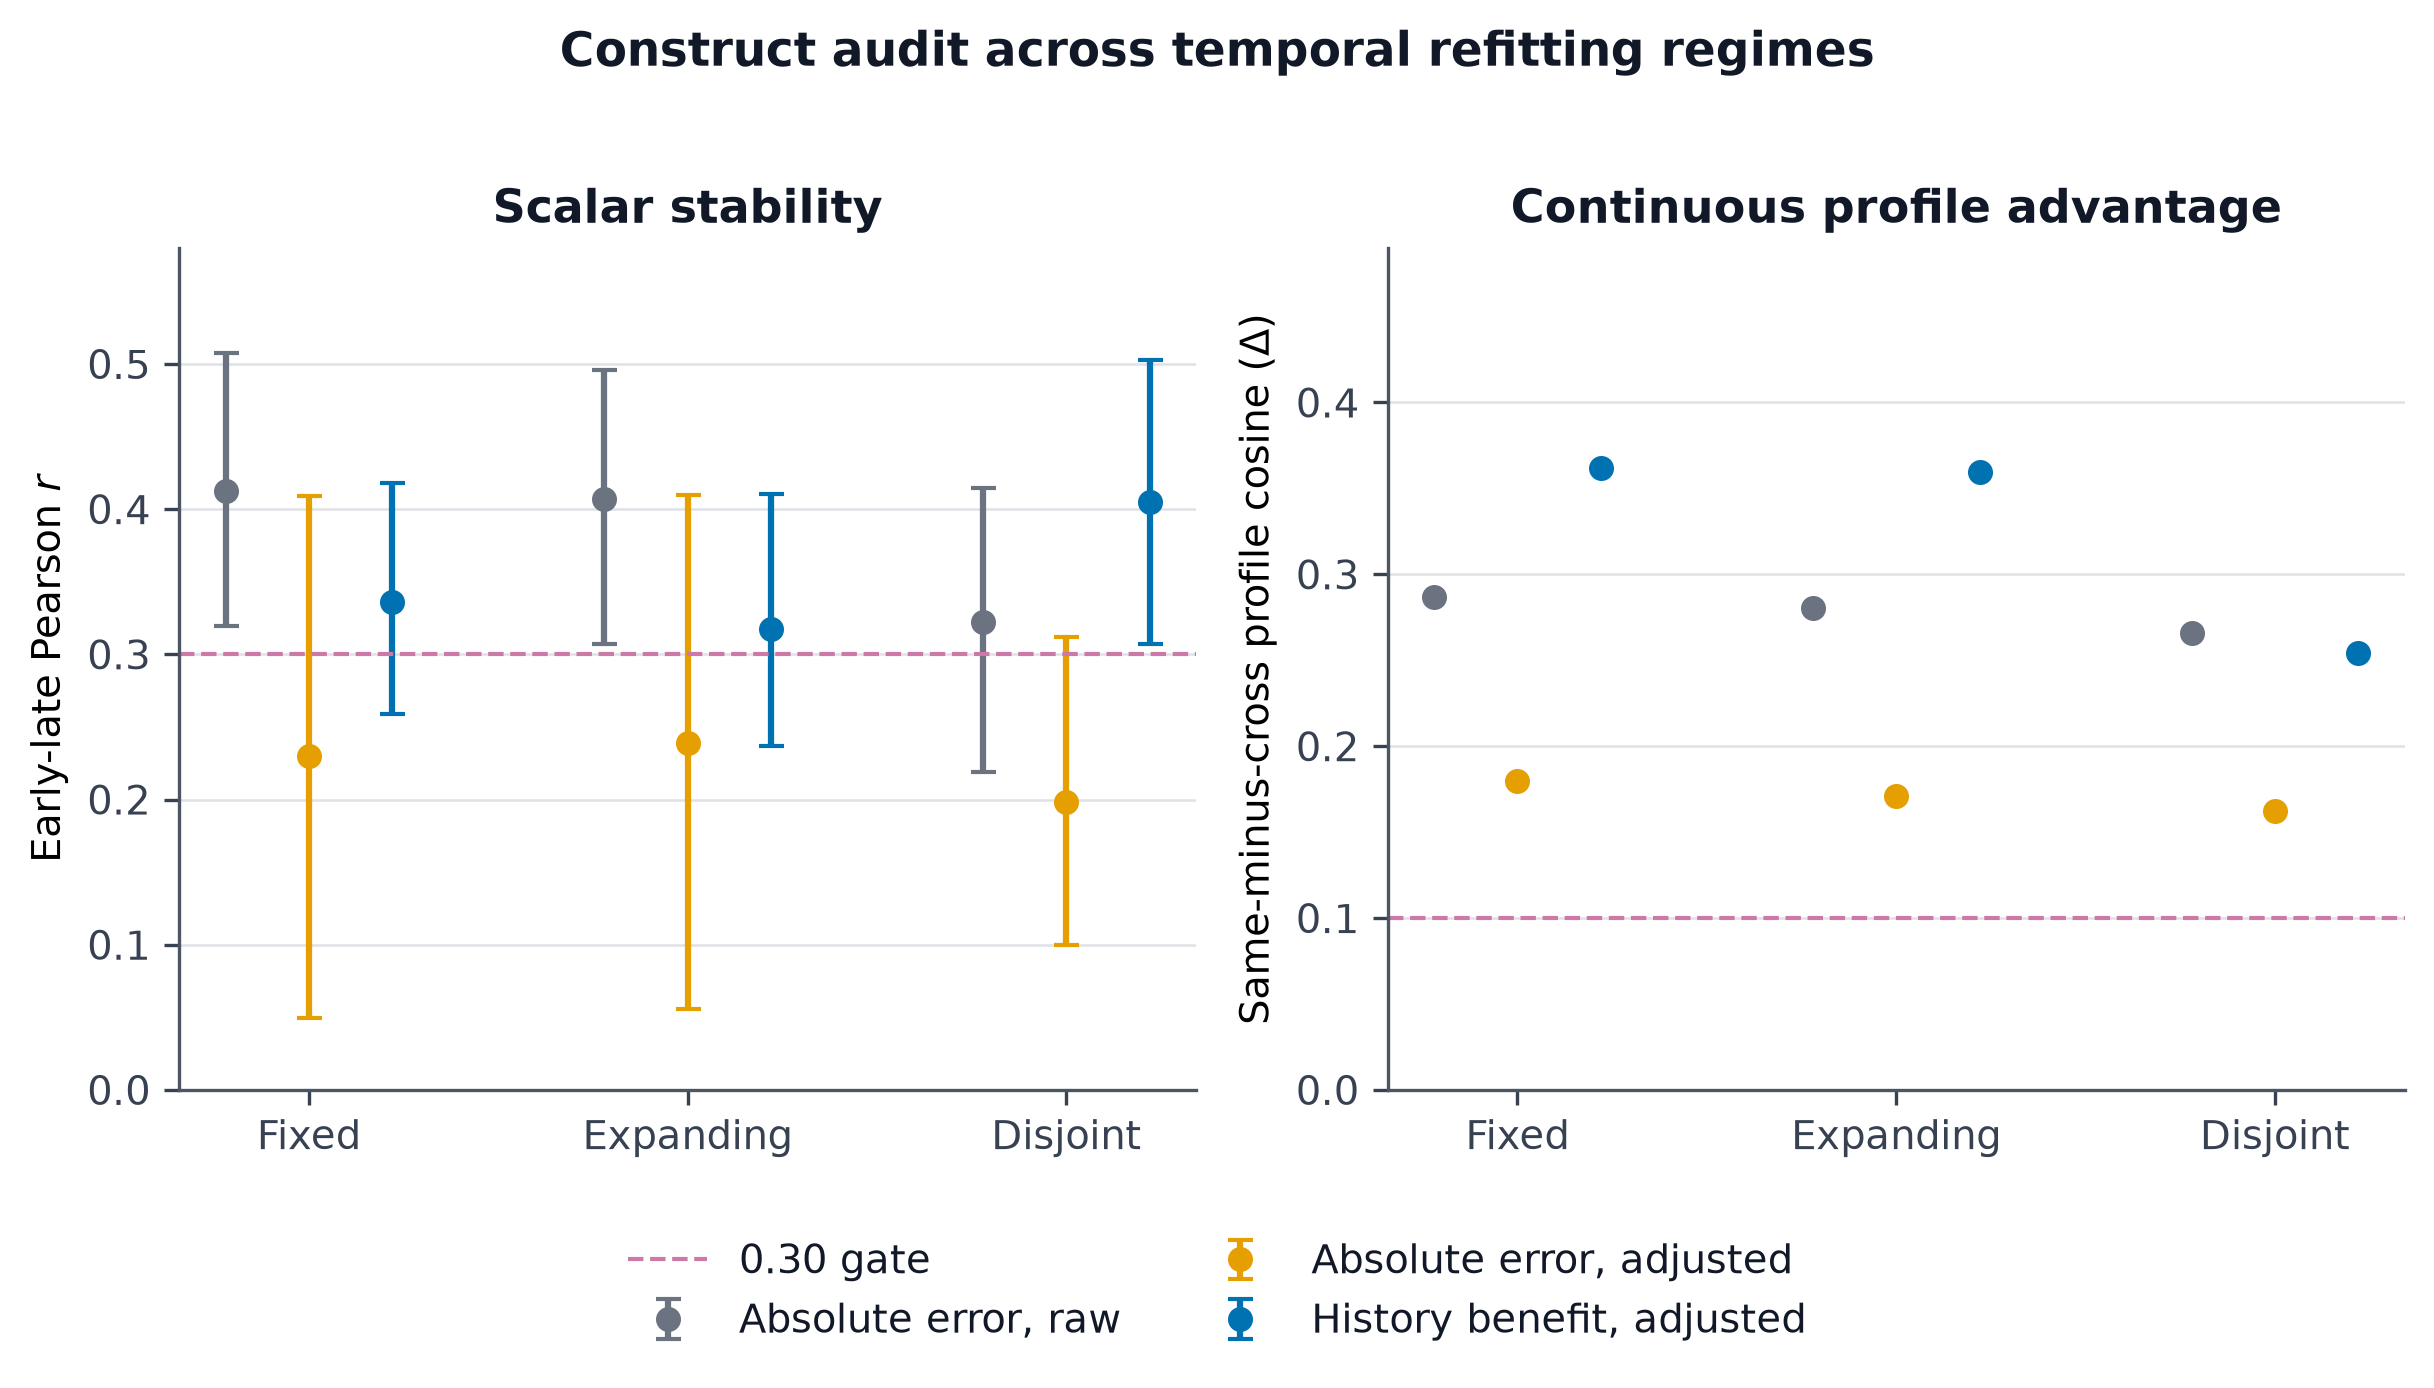
\includegraphics[width=\textwidth]{forecastability_construct_audit.png}
\caption[Forecastability construct audit across refitting regimes]{Construct audit for the core eight-domain sample. Scalar stability uses
521 trajectories in fixed and expanding regimes and 499 in the disjoint regime;
error bars are trajectory-bootstrap 95\% intervals. Profile advantage is the
same-minus-matched-cross early/late cosine difference. The magenta lines show the
project-specific 0.30 scalar criterion and 0.10 profile criterion. Adjusted rows control
test-window target standard deviation and marginal quintile entropy. Profile tests
used 10,000 permutations and had $p<0.001$.}
\label{fig:construct-audit}
\end{figure}

\begin{table}[H]
\centering
\caption[Core construct-audit results]{Core construct-audit results. The adjusted absolute-error point estimate fails the
0.30 gate in every regime. Relative history benefit is model-relative and remains
subject to the stronger controls in \cref{tab:stronger-controls}.}
\label{tab:construct-audit}
\resizebox{\textwidth}{!}{%
\begin{tabular}{@{}llS[table-format=1.3]lS[table-format=1.3]l@{}}
\toprule
Measure & Regime & {Degree $r$} & 95\% CI & {Profile $\Delta$} & Status \\
\midrule
Absolute error, raw & Fixed & 0.412 & [0.316, 0.501] & 0.287 & Raw gate met \\
 & Expanding & 0.407 & [0.307, 0.496] & 0.280 & Raw gate met \\
 & Disjoint & 0.322 & [0.219, 0.414] & 0.266 & Raw gate met \\
\addlinespace
Absolute error, SD/entropy adjusted & Fixed & 0.230 & [0.049, 0.409] & 0.180 & Scalar \failed \\
 & Expanding & 0.239 & [0.056, 0.409] & 0.171 & Scalar \failed \\
 & Disjoint & 0.198 & [0.100, 0.312] & 0.162 & Scalar \failed \\
\addlinespace
History benefit, SD/entropy adjusted & Fixed & 0.336 & [0.259, 0.418] & 0.362 & \exploratory \\
 & Expanding & 0.317 & [0.237, 0.410] & 0.360 & \exploratory \\
 & Disjoint & 0.405 & [0.307, 0.503] & 0.254 & \exploratory \\
\bottomrule
\end{tabular}}
\end{table}

The construct audit is a specification correction rather than a rescue of the
initial scalar. Global-SD-normalized absolute error mainly measured stable behavioral
variability, so it should not be named a distinct forecastability phenotype. The
positive residual association is compatible with a smaller remaining signal, but it
neither met the historical point-estimate rule nor isolated a distinct construct.

Equation~\ref{eq:skill} is the preferable operationalization for asking whether
history helps relative to a calendar comparator. Under SD/entropy adjustment its
scalar correlations were 0.336, 0.317, and 0.405 across fixed, expanding, and
disjoint regimes. Those estimates do not validate $S$ as a trait: stronger
training-window and sequence controls attenuated the scalar, and the measure remains
comparator-dependent. Only its continuous cross-domain profile is retained as a
post-hoc lead.

\subsection{The continuous profile remained a post-hoc lead}

Relative history benefit was less coupled to standard deviation than raw error at
the person-average level ($r=-0.268$), but it still correlated with marginal entropy
($r=-0.518$). Its raw split-half stability was 0.484, 0.473, and 0.445 under fixed,
expanding, and disjoint regimes.

The scalar did not survive every stronger control. Training-window moment adjustment
produced $r=0.323$, 0.263, and 0.322; the expanding value failed the 0.30 gate.
Sequence-proxy adjustment produced $r=0.240$, 0.219, and 0.246; all failed. The
history-benefit scalar is therefore not a robust phenotype.

The continuous profile was more consistent. Same-minus-cross profile advantages
remained above 0.10 after three types of adjustment
(\cref{tab:stronger-controls}). All listed tests used 10,000 within-cohort
permutations and had $p<0.001$.

\begin{table}[H]
\centering
\caption[Continuous profile under stronger controls]{Post-hoc continuous profile of pooled relative history benefit under
stronger controls. Values are same-minus-matched-cross cosine differences. Sample
sizes for sequence adjustment are 439, 439, and 425 trajectories for fixed,
expanding, and disjoint regimes.}
\label{tab:stronger-controls}
\resizebox{\textwidth}{!}{%
\begin{tabular}{@{}lSSS l@{}}
\toprule
Adjustment & {Fixed $\Delta$} & {Expanding $\Delta$} & {Disjoint $\Delta$} & Status \\
\midrule
Test-window SD and marginal entropy & 0.362 & 0.360 & 0.254 & \exploratory \\
Training-window SD and marginal entropy & 0.354 & 0.311 & 0.217 & \exploratory \\
Sequence-order proxies & 0.314 & 0.308 & 0.202 & \exploratory \\
\bottomrule
\end{tabular}}
\end{table}

The identity sensitivity excluded every trajectory flagged as a
possible cross-year repeat. For the core, standard-deviation/entropy-adjusted
history-benefit profile, 232 fixed and expanding trajectories and 215 disjoint
trajectories remained. Same-minus-matched-cross profile advantages were 0.338,
0.333, and 0.242, respectively (all $p=0.002$, 500 permutations). This conservative
exclusion shows that known repeat candidates did not drive the result, while the
missing cross-year identifier still limits the unit to a person-year trajectory.

The surviving secondary result is therefore a continuous within-trajectory profile
of where pooled history features transfer relative to pooled calendar features. It
requires replication with recoverable identities and independent data.

\section{RQ4: mechanism, typology, and feasibility}

\subsection{Own-domain multiscale history carried the profile}

After test-window standard-deviation and marginal-entropy adjustment, 7/14-day
means, their recent-history combination, the 42-day fingerprint, and all own-domain
history passed the exploratory scalar and profile gates across the three regimes.
Yesterday alone did not pass the scalar gate in every regime
(\cref{fig:feature-families}).

\begin{figure}[H]
\centering
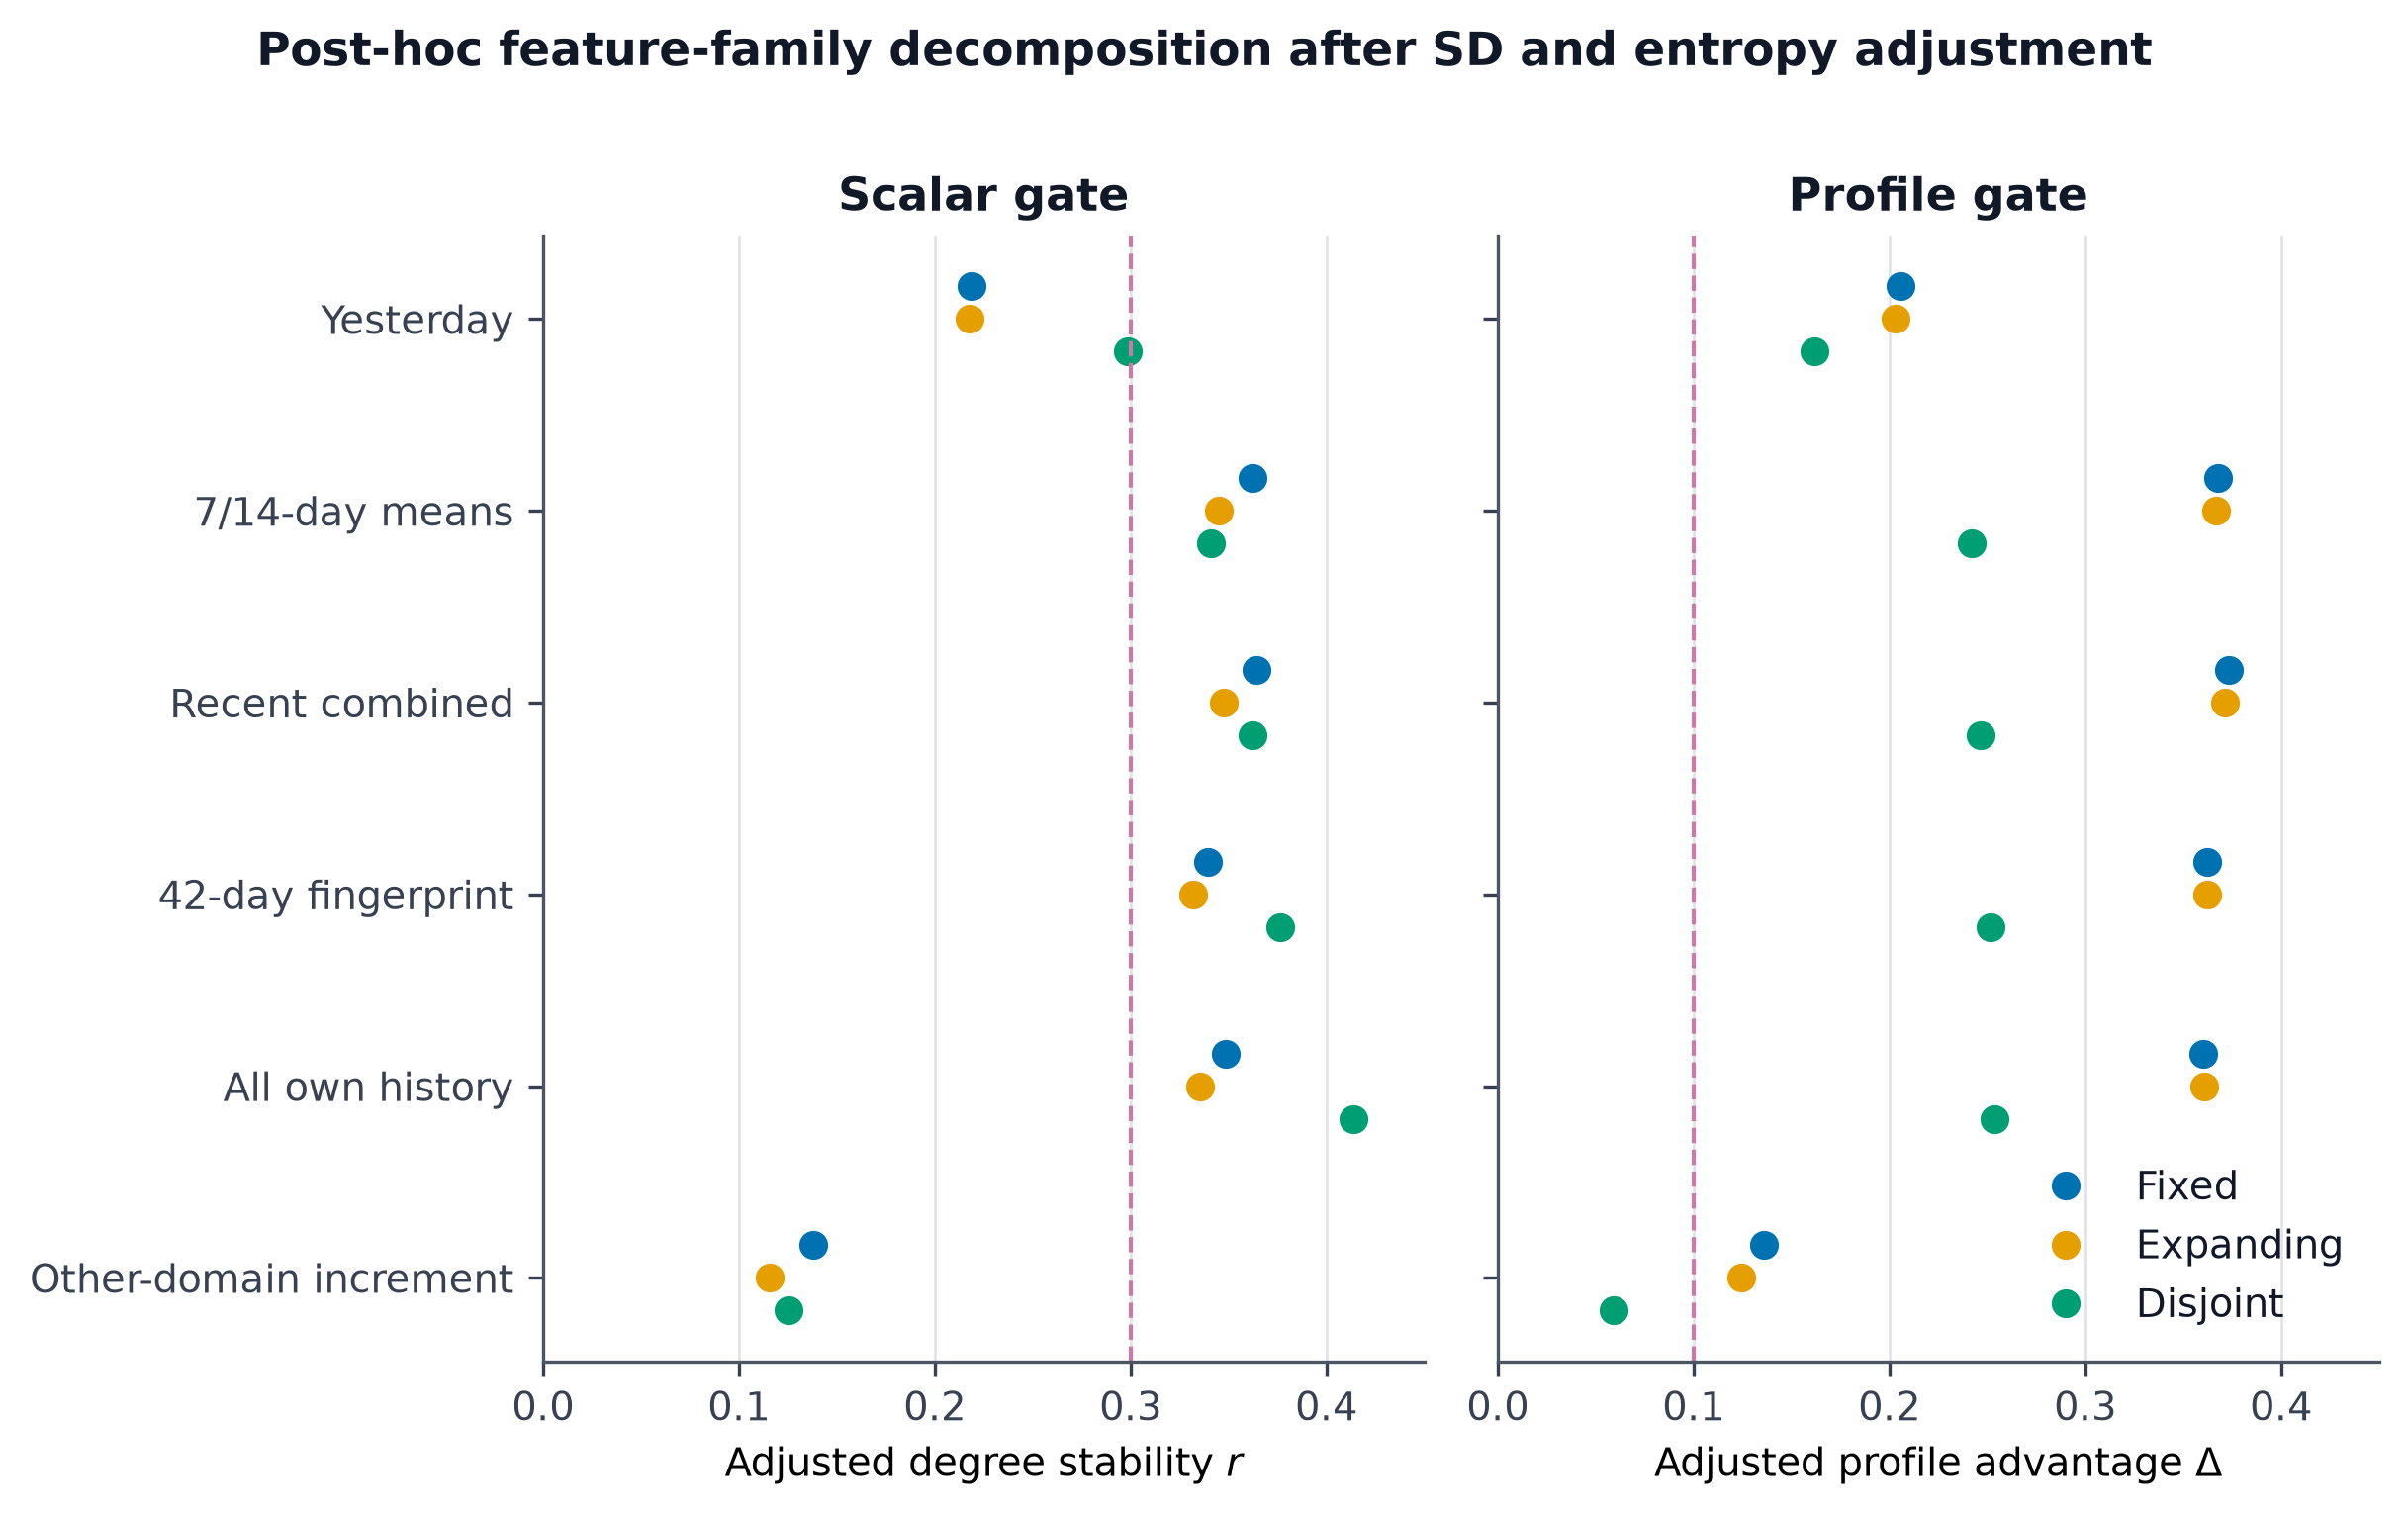
\includegraphics[width=\textwidth]{feature_family_decomposition.png}
\caption[Post-hoc feature-family decomposition]{Post-hoc feature-family results after target-specific test-window standard
deviation and marginal-entropy adjustment. Degree stability is early/late Pearson
$r$; profile advantage is the same-minus-matched-cross cosine difference. Magenta
lines show exploratory 0.30 and 0.10 gates. Fixed, expanding, and disjoint core
samples contain 521, 521, and 499 trajectories. Secondary profile tests used 500
permutations and reached the resolution floor $p\leq0.002$.}
\label{fig:feature-families}
\end{figure}

The feature families overlap. Recent history and the 42-day fingerprint produced
similar aggregate errors, and their combination yielded only a small additional
change. The analysis does not identify one exclusive mechanism.

\subsection{Cross-domain coupling was unsupported}

Adding other-domain recent histories worsened aggregate held-out MAE by 0.47\%,
0.44\%, and 0.42\% under fixed, expanding, and disjoint refitting. It improved four,
four, and two of eight targets. The cross-domain performance gate required an
aggregate improvement and at least six improved targets. It failed in every regime.

The surviving profile should therefore not be explained as cross-domain behavioral
coupling. The supported description is multiscale own-domain pooled-model
transferability under the tested controls.

\subsection{No discrete routine types replicated}

No $k$ from 2 through 5 passed the leave-one-cohort-out typology gate
(\cref{fig:typology}). Median ARI ranged from 0.034 to 0.066 for fixed models and
0.028 to 0.057 for disjoint models. Every candidate had zero held-out cohorts that
met the joint rule.

\begin{figure}[H]
\centering
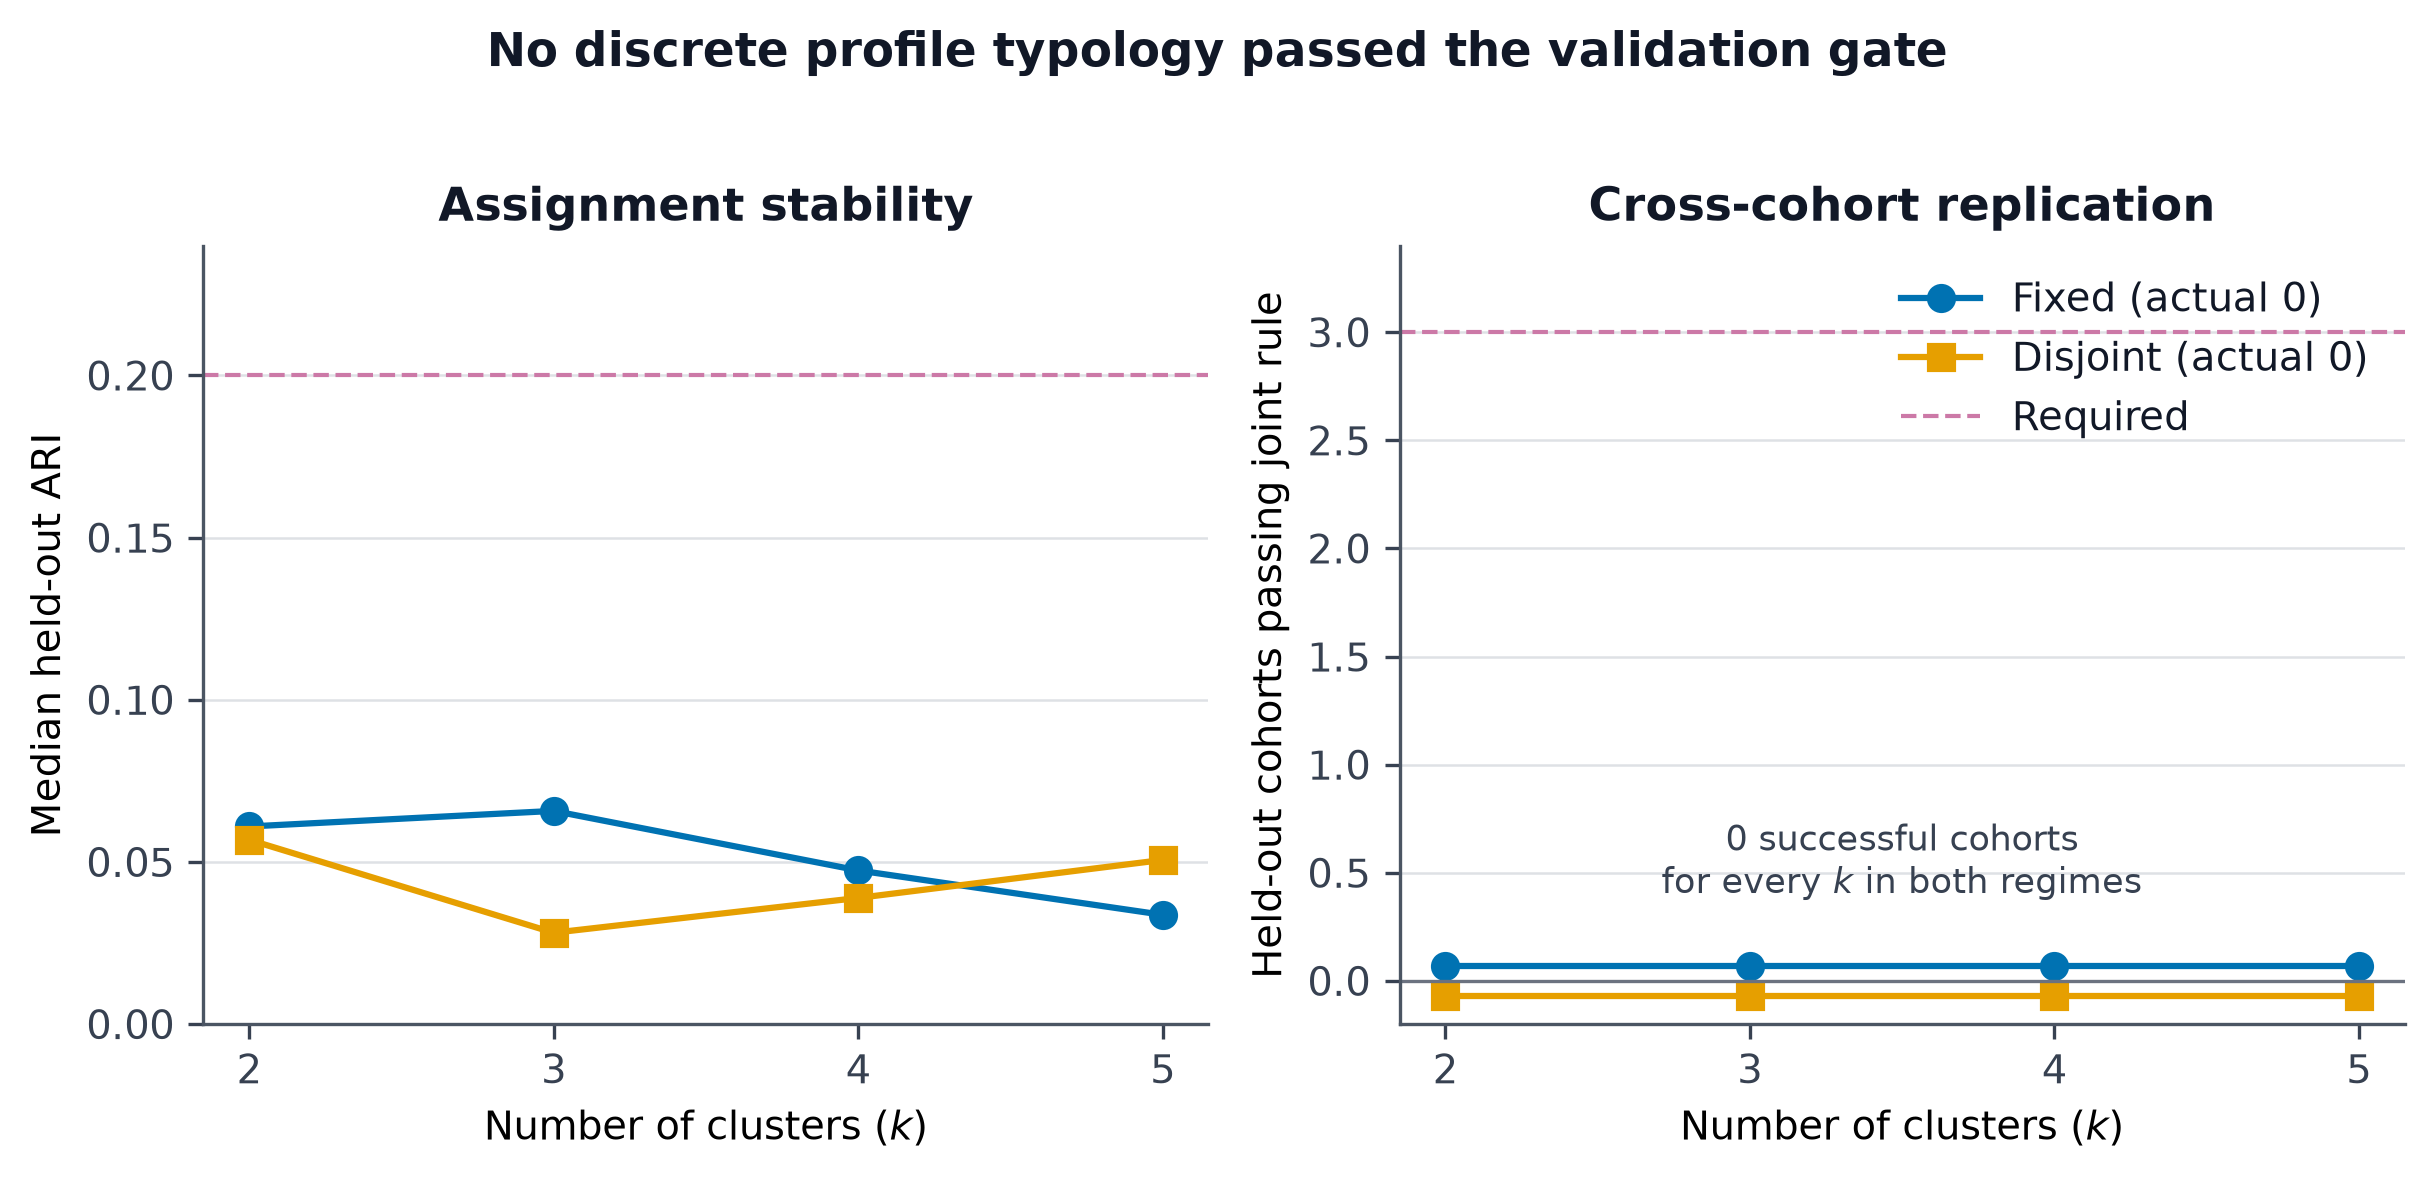
\includegraphics[width=\textwidth]{typology_validation.png}
\caption[Leave-one-cohort-out typology validation]{Post-hoc leave-one-cohort-out validation of spherical profile clustering.
The left panel shows median adjusted Rand index across held-out cohorts; the right
panel shows the number of held-out cohorts meeting the joint stability rule. Magenta
lines mark the exploratory requirements of ARI $>0.20$ and at least three successful
cohorts. Both right-panel series equal zero for every $k$; their markers are offset
slightly only so both series remain visible. No $k=2,\ldots,5$ passed in fixed or
disjoint regimes.}
\label{fig:typology}
\end{figure}

Descriptive centroids can be given intuitive labels, but participants did not retain
those assignments. The report therefore does not define sleep-, activity-, or
screen-anchored behavioral types.

\subsection{Personalization study stopped before modeling}

The preferred branch of the outcome-blind feasibility audit retained only mobility
and phone-interaction families. The selected mobility target had a minimum of 36
eligible person-targets across institute-years and 329 in total. The selected
phone-interaction target also had a minimum of 36 and 327 in total. Physical activity
and sleep had minima of 14 and 13, below the required 30. The reduced branch retained
no family.

The contract required an allowed multi-family branch. None remained, so the selected
branch and selected targets were empty. No model, prediction, loss, or outcome
comparison was run. The correct status is \stopped\ at a feasibility boundary, not
a personalization null.

\section{Secondary and exploratory findings}

No corrected association with conscientiousness, extraversion, or social fit passed
H3. The test had limited sensitivity for effects near the 0.10 gate, so the result is
\inconclusive. It does not establish independence from personality.

The common-distress follow-up was post-hoc and cross-sectional. The original
controlled estimate was $r=-0.178$ for 518 trajectories. Direct target standard
deviation control gave $r=-0.140$, with cohort values ranging from approximately
0.008 to $-0.342$. Because the estimates were heterogeneous and unreplicated, they
are excluded from the abstract and central conclusion.

\chapter{Discussion and Lessons Learned}
\label{ch:discussion}

\section{Evaluation against the research questions}

RQ1 found no detectable passive increment over label history and no moderate shared
within-trajectory ranking effect; sparse trajectories left subtle heterogeneous and
individual effects unresolved. Cross-family outcomes still overlapped substantially.
RQ2 established direct-behavior continuity under pooled chronological models;
calendar-only performance was weak and simple same-channel history supplied most of
the lift. RQ3 identified a specification error in global-SD-normalized
forecastability and retained only a corrected, comparator-relative continuous
profile as a post-hoc lead. RQ4 found no support for cross-domain improvement or
discrete typology, while the separate personalization design stopped before model
fitting.

\section{Implication for passive-sensing target choice}

The project supports a limited but useful conclusion. In this GLOBEM comparison,
prior self-report history was more predictive of the depression label than the
tested passive features. The repeated psychological columns also shared substantial
variance. A passive classifier can therefore appear effective without adding new
measurement of a named psychological state.

This result changes the evaluation standard. A current-day passive model should not
be judged only against chance or another passive model. It should be judged against
the person's available label history. A multi-construct dataset should also examine
whether the target is empirically distinct from related outcomes.

Passive features may still support monitoring, context, adherence, or longer
within-person studies, but a state-inference claim must first demonstrate value over
the person's available label history.

\section{What forecastability measured}

The scalar audit identified a specification error. Equation~\ref{eq:forecastability}
normalized absolute history-model error by a global target standard deviation. Its
split-half correlation of 0.412 was reproducible under refitting, but the $-0.912$
association with person-level behavioral standard deviation showed that it mostly
ranked low-variance trajectories. Reproducibility therefore did not confer construct
validity.

Equation~\ref{eq:skill} corrects the principal defect by comparing history-model and
calendar-model errors within the same trajectory, target, and window. This makes it
appropriate for the narrower question of incremental historical information. It is
still comparator-dependent, and pooled coefficients measure transferability rather
than idiographic learnability. Its scalar form also failed stronger sequence
controls; only the continuous history-benefit profile remains as a post-hoc lead.

The original H1 rule adds a second lesson. The adjusted estimate of $r=0.230$ with
95\% CI $[0.049,0.409]$ failed the point-estimate threshold but remained compatible
with effects on either side of 0.30. Future work should pre-specify an interval-based
minimum effect or an equivalence/non-inferiority test.

\section{Meaning of the continuous domain profile}

The post-hoc profile result is narrower. It states that the pattern of domains in
which a pooled history model outperformed a pooled calendar model was more similar
within a person-year trajectory than across matched trajectories. This held after
the tested moment and sequence controls.

Three boundaries are essential:

\begin{enumerate}
  \item the models use population-average coefficients, so the profile measures
  transferability rather than personal-model learnability;
  \item the unit is a person-year trajectory, not a cross-year identified person;
  and
  \item the result was developed post-hoc in one dataset and requires prospective
  external replication.
\end{enumerate}

Within these boundaries, the continuous profile is a reasonable replication target
and appears to use multiscale own-domain history. No clinical or personality label is
assigned to it.

\section{Negative results as design information}

The project produced several useful negative results. Richer passive context and
small neural models did not rescue psychological-label prediction. Cross-domain
histories did not improve the behavior forecast, and the 42-day plus partial-day
terms added little on average beyond simple recent same-channel history. Discrete clusters did not replicate
across cohorts. The personalization design did not have sufficient balanced data for
its required multi-family comparison.

Together, these results favor simple baselines, prospective evaluation, continuous
profiles, and feasibility checks before model fitting.

\section{Applied baseline lesson}

The GLOBEM analyses and the Android pilot share neither participants, features, nor
models, but they expose the same evaluation error at different stages of a system.
The GLOBEM psychological models required comparison with prior labels, and the
behavior forecasts required temporal comparators; in the single-user pilot in
\cref{app:android-pilot}, an app-based score ranked adjustment events moderately well
(AUROC 0.740), yet both tested action policies produced higher error than leaving the
setting unchanged. Predictive discrimination is insufficient evidence for
intervention when false actions carry asymmetric cost, so policy evaluation must
include a no-action baseline. A later saved-model reconstruction on the same phone
showed exploratory enrichment of observed adjustment events among selected sessions,
but its day-clustered interval for all-session error improvement included zero
(\cref{sec:september-volume-followup}).

\section{Project-execution lessons}

\subsection{Strong baselines should be implemented early}

The label-history control changed how earlier passive scores were interpreted. For
longitudinal labels, prior-label and prevalence baselines belong in the first test.

\subsection{Construct audits should follow prediction tests}

Prediction and temporal reproducibility do not validate a new construct. Variance,
entropy, missingness, and comparator behavior should be tested early.

\subsection{Stopping rules protect follow-up studies}

The outcome-blind personalization audit stopped an underpowered, unbalanced design
before model fitting or post-hoc redefinition of its target set.

\subsection{Confirmatory status and multiplicity}

The analyses mix project-specified and post-hoc tests. Post-hoc $p$-values remain
exploratory, not confirmatory or family-wise error-controlled.

\section{Threats to validity}

\textbf{Population and season.} GLOBEM contains campus cohorts observed during
spring academic terms. Results may not generalize to clinical, community, older, or
seasonally different populations. Shared academic calendars may contribute to
behavioral continuity.

\textbf{Identity.} Cross-year identity is incomplete. The report cannot establish a
stable person-level trait across years. Excluding repeat candidates is conservative
but does not reconstruct the missing identity clusters.

\textbf{Released aggregates.} Models use RAPIDS aggregate features rather than raw
sensor streams. Results depend on feature extraction, missingness, platform, target
definition, issue time, and model class.

\textbf{Time scale.} Early and late windows span weeks, not years or major life
changes. Stability over these windows is not long-term reliability.

\textbf{Internal gates.} The 0.30 and 0.10 thresholds were recorded within the
project and are not universal standards. Their repository record is not independently
timestamped before analysis.

\textbf{Entropy proxies.} Marginal quintile entropy and short discretized sequence
metrics do not estimate a theoretical predictability ceiling. Their estimates are
sensitive to window length and discretization.

\textbf{Pooled comparator.} Relative history benefit depends on both a pooled
history model and a pooled calendar model. Normalized calendar MAE varied modestly
across cohorts. The score is not comparator-free.

\textbf{Post-hoc development and uncertainty.} The profile, feature-family,
sequence, typology, and distress analyses followed earlier results; their thresholds
do not confer external confirmation. Aggregate behavior means have no single common
confidence interval, some secondary profile tests used only 500 permutations, and
H3 had limited power for small corrected associations.

\chapter{Conclusion and Future Work}
\label{ch:conclusion}

\section{Conclusions}

This project gives four direct conclusions.

\begin{enumerate}
  \item \textbf{Screening-label validity is the primary result.} The released target
  mixes PHQ-4, a year-1 PANAS-derived rule, and an end-term BDI-II observation; it is
  a screening proxy rather than a diagnosis. It was positive in 45.4\%/47.7\% of
  chronological train/test rows. Prior positive-label history achieved AUROC 0.844. Adding
  current-day or historical passive features produced 0.840 and 0.841, with
  clustered increment intervals that included zero. The primary within-person AUROC
  was 0.514 (95\% CI $[0.474,0.556]$). The tested passive features therefore had no
  detectable aggregate or moderate shared within-person increment. The available
  trajectories had 80\% simulated power near a shared AUROC of 0.56, but remained
  insufficient for subtle, heterogeneous, or individual effects. Nonredundant
  psychological construct pairs still showed median absolute correlation 0.590.

  \item \textbf{Direct behavior exhibits prospective persistence.} Calendar-only
  models had mean tomorrow $R^2=-0.007$ and AUROC 0.544. Recent same-channel history
  raised these to 0.244 and 0.767, while the complete model reached 0.272 and 0.788.
  Its medians were $R^2=0.260$ (target range $-0.113$ to 0.637) and AUROC 0.795
  (range 0.699--0.884). Simple history therefore supplied most forecast value; the
  result is continuity of observed behavior, not evidence that a rich fingerprint
  is necessary.

  \item \textbf{The original scalar was mis-specified.} Global-SD-normalized
  forecastability correlated $-0.912$ with behavioral standard deviation and mainly
  ranked low-variance trajectories. Its adjusted split-half estimate was $r=0.230$
  (95\% CI $[0.049,0.409]$), below the project-specified 0.30 point gate. A corrected
  score compared history-model error with calendar-model error within the same
  trajectory, target, and window, but remained comparator-dependent.

  \item \textbf{A continuous corrected profile remains a post-hoc lead.} The pattern
  of domain-specific relative history benefit survived the tested moment and
  sequence controls. Cross-domain coupling and discrete types were unsupported. The
  profile measures pooled-model transferability, not idiographic learnability or a
  stable cross-year phenotype.
\end{enumerate}

\section{Recommended replication study}

The next study should test the continuous profile in an independent dataset with
longer trajectories and recoverable person identifiers. Its contract should be
timestamped before outcome analysis. The study should compare:

\begin{enumerate}
  \item pooled history models;
  \item hierarchical or mixed-effects models; and
  \item separately fitted person-specific models.
\end{enumerate}

The primary question should be whether the same domain profile remains within the
same person across independent periods and model classes. Variability, training-window
moments, missingness, weekday structure, and preselected sequence metrics should be
controls from the start.

\section{Requirements before personalization}

The stopped feasibility audit should be repeated only when the candidate dataset
meets its frozen per-cohort and total eligibility requirements. A revised contract
may use fewer target families, but that change must be justified before inspecting
model outcomes. Feasibility and effect estimation must remain separate phases.

\section{Final project statement}

The project does not support an autonomous passive detector of a named psychological
state, a scalar routine phenotype, or discrete routine types. It supports a clear
measurement rule: compare passive models with label history, forecast direct behavior
prospectively, and audit prediction-derived scores against simpler behavioral
constructs. That rule is the defensible contribution of the work.

Across the project, the resulting baseline hierarchy is: psychological-label models
must beat label history and behavioral forecasts must beat temporal comparators.
The separate single-user pilot in \cref{app:android-pilot} illustrates the analogous
decision-system requirement that an intervention policy must beat no action.

\clearpage
\bibliographystyle{plainnat}
\bibliography{references}

\appendix

\chapter{Per-Target Behavioral Forecast Results}
\label{app:rq2-targets}

The aggregate RQ2 summaries conceal substantial target heterogeneity. For the full
evening model, tomorrow $R^2$ ranged from $-0.113$ to 0.637 and tomorrow AUROC from
0.699 to 0.884. \Cref{tab:rq2-per-target} therefore reports every target for both
horizons. Target names describe released aggregate channels and should not be read
as psychological constructs.

\footnotesize
\begin{longtable}{@{}L{0.28\textwidth}C{0.14\textwidth}C{0.14\textwidth}C{0.14\textwidth}C{0.14\textwidth}@{}}
\caption[RQ2 per-target results]{Per-target held-out performance for the full evening model. The model combines recent history, the 42-day fingerprint, and the current partial day. Values are descriptive across heterogeneous direct-behavior targets.}\label{tab:rq2-per-target}\\
\toprule
Target & \makecell{Tomorrow\\$R^2$} & \makecell{Tomorrow\\AUROC} & \makecell{Seven-day\\$R^2$} & \makecell{Seven-day\\AUROC} \\
\midrule
\endfirsthead
\multicolumn{5}{l}{\textit{Table \thetable\ continued}}\\
\toprule
Target & \makecell{Tomorrow\\$R^2$} & \makecell{Tomorrow\\AUROC} & \makecell{Seven-day\\$R^2$} & \makecell{Seven-day\\AUROC} \\
\midrule
\endhead
\midrule
\multicolumn{5}{r}{\textit{Continued on next page}}\\
\endfoot
\bottomrule
\endlastfoot
Sleep Efficiency & 0.637 & 0.782 & 0.824 & 0.901 \\
Bluetooth Unique Devices & 0.561 & 0.882 & 0.633 & 0.935 \\
Wifi Unique Devices & 0.520 & 0.866 & 0.694 & 0.935 \\
Screen Unlock Count & 0.355 & 0.884 & 0.656 & 0.940 \\
Outgoing Call Count & 0.312 & 0.778 & 0.546 & 0.848 \\
Steps Sum & 0.299 & 0.829 & 0.660 & 0.925 \\
Active Duration & 0.265 & 0.811 & 0.645 & 0.903 \\
Location Home Time & 0.261 & 0.807 & 0.155 & 0.843 \\
Incoming Call Count & 0.259 & 0.747 & 0.530 & 0.846 \\
Screen Unlock Duration & 0.258 & 0.833 & 0.613 & 0.919 \\
Significant Places & 0.247 & 0.726 & 0.463 & 0.833 \\
Location Entropy & 0.243 & 0.732 & 0.385 & 0.809 \\
Sedentary Duration & 0.172 & 0.812 & 0.668 & 0.902 \\
Sleep Duration & 0.037 & 0.710 & 0.415 & 0.818 \\
Sleep In Bed & 0.031 & 0.703 & 0.354 & 0.802 \\
Location Distance & -0.113 & 0.699 & -0.143 & 0.773 \\
\end{longtable}
\normalsize


\chapter{Neural Model-Class Diagnostics}
\label{app:neural-diagnostics}

Two small neural classifiers were evaluated during model exploration. The cleanest
model-class diagnostic was a tabular MLP using the same 196 RAPIDS 7/14-day history
features and outer evaluation splits as the random-forest history baseline. Its
inner validation respected the outer regime: later rows within each training
trajectory were used for within-user validation, whereas complete user trajectories
sampled within institute-year were used for held-out-user validation.

\begin{table}[H]
\centering
\scriptsize
\setlength{\tabcolsep}{3pt}
\caption[Neural model-class diagnostics]{Single-run neural diagnostics and the
random-forest history comparator. ``Fit/val/test'' reports row counts. Validation
AUROC is absent for the random forest because it was fitted on the complete outer
training block. Metrics are shown to three decimals; full-precision outputs are
retained in the statistical supplement.}
\label{tab:neural-diagnostics}
\begin{tabular}{@{}llllrrrr@{}}
\toprule
Model & Input & Split & Fit/val/test & \makecell{Val.\\AUROC} &
\makecell{Test\\AUROC} & \makecell{Macro-\\F1} & \makecell{Bal.\\acc.} \\
\midrule
RF & RAPIDS history & Within user & 5,213/--/2,927 & -- & 0.691 & 0.640 & 0.642 \\
MLP & RAPIDS history & Within user & 4,397/816/2,927 & 0.709 & 0.619 & 0.579 & 0.580 \\
LSTM & Raw 14-day sequence & Within user & 4,431/782/2,927 & 0.664 & 0.622 & 0.596 & 0.597 \\
\addlinespace
RF & RAPIDS history & Held-out users & 6,063/--/2,077 & -- & 0.577 & 0.548 & 0.548 \\
MLP & RAPIDS history & Held-out users & 5,157/906/2,077 & 0.547 & 0.559 & 0.536 & 0.536 \\
LSTM & Raw 14-day sequence & Held-out users & 5,153/910/2,077 & 0.698 & 0.553 & 0.541 & 0.542 \\
\bottomrule
\end{tabular}
\end{table}

The MLP is the matched-input diagnostic, but not an identical-training-exposure
comparison: it reserved part of the outer-training pool for checkpoint selection,
whereas the random forest used the complete outer-training block. It trailed the
random forest by 0.071 AUROC within user and by 0.018 on held-out users. The saved
LSTM run used 100 all-day sequence features plus their missingness indicators rather
than the RAPIDS history vector. Its result files also predate the validation-hygiene
rewrite and contain no retained split-summary artifact, so it is reported only as a
legacy exploratory baseline, not as a matched or hygienic-validation comparison.

No repeated-seed distribution, neural confidence interval, or systematic
hyperparameter search was run. The supported conclusion is narrow: the tested small
MLP did not improve on the random-forest history baseline under the same feature
representation and outer split. These runs do not establish that neural models are
generally inferior for passive-sensing data.

\chapter{Independent Android Self-Instrumentation Pilot}
\label{app:android-pilot}

\section{Scope, collection, and privacy}

As a separate applied work package, the author designed, implemented, and operated
a custom Android logger on their own phone. It recorded 525 listening sessions over
37 calendar days, linking generic app identity, output device, time, initial and
settled media volume, and provenance evidence for matched hardware-key changes. The
author was both system designer and the sole observed user, so reactivity and
experimenter-participant coupling are unavoidable. This pilot is not part of the
GLOBEM research questions, a transfer experiment, or a population study.

Exact app and package identities and raw session logs remain private. The report
uses generic app references and only aggregate counts, metrics, contracts, and
de-identified displays. No third-party participant was observed, and no suggestion
or automatic actuation was enabled.

\section{Frozen evaluation and developmental model}

A protocol activation record froze the eligible collection window and evaluator.
After pre-activation sessions and sessions with context changes in the evaluation
window were excluded, 258 sessions remained. The first 180 sessions were used for
estimation and the final 78 as a future test block; 33 test sessions contained a
matched hardware-key adjustment.

The developmental two-stage mechanism was formulated after the completed
prospective block and is therefore post-hoc. Stage one estimated adjustment
probability from generic app identity using beta-smoothed training rates. Stage two
used only adjustment-positive sessions and estimated settled volume from
hierarchical training medians. Its primary specification used device and a
three-hour time bucket while excluding app identity and current volume. The
end-to-end policy applied the destination estimate when the stage-one probability
was at least 0.50 and otherwise retained the current volume. The primary policy
comparator was no action: always retain the current volume. Paired uncertainty used
2,000 session-level bootstrap resamples.

\begin{figure}[H]
\centering
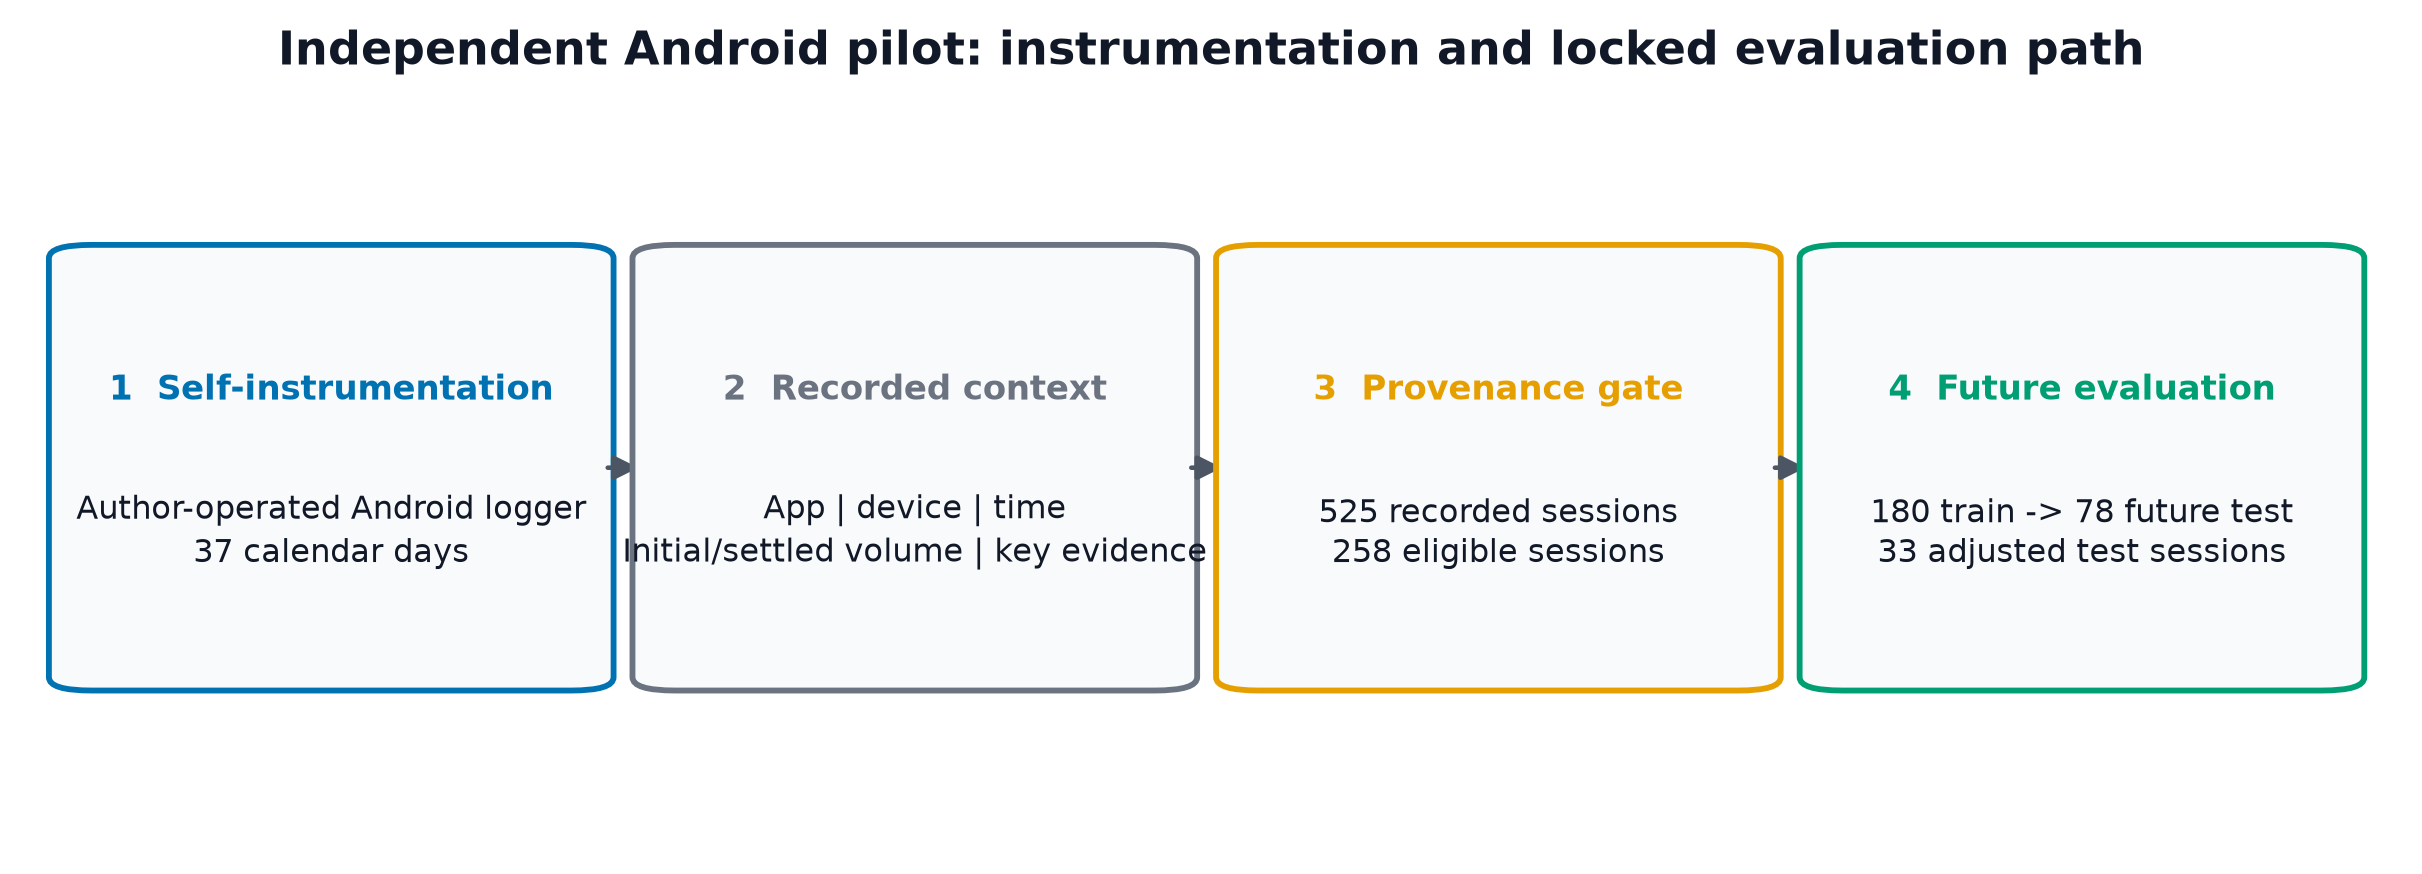
\includegraphics[width=\textwidth]{android_pilot_workflow.png}
\caption[Android self-instrumentation workflow]{Independent Android pilot workflow.
The author implemented and operated the logger, recorded 525 sessions over 37
calendar days, froze a provenance-aware eligible window, and evaluated 258 eligible
sessions chronologically. The pilot is a post-hoc single-user applied work package,
not a GLOBEM replication or population study.}
\label{fig:android-workflow}
\end{figure}

\section{Results}

Generic app identity moderately ranked whether an adjustment occurred in the 78
future test sessions: AUROC was 0.740, Brier score 0.203, and balanced accuracy
0.670 at the 0.50 threshold. The threshold produced 31 true positives and two false
negatives, but also 27 false positives among 45 sessions with no observed
adjustment, giving specificity 0.400. Ranking performance therefore did not by
itself establish a useful action rule.

The destination-volume hypothesis failed its developmental decision rule.
Device and time without app identity had MAE 21.73 on the 33 adjustment-positive
test sessions, 5.70 points worse than the global median (95\% paired-bootstrap
interval 2.55 to 8.82). The app-aware sensitivity reached MAE 14.53, but its
1.50-point difference from the global median had interval $[-4.21,1.50]$ and did
not meet the recorded 10\% practical-effect rule. Because the paired empirical
bootstrap resamples only 33 adjusted sessions, its distribution is discrete; the
upper 97.5th percentile equalling 1.50 is the computed quantile, not a transcription
error.

\begin{table}[H]
\centering
\small
\caption[Android destination-volume results]{Destination-volume MAE on the 33
adjustment-positive future test sessions. Lower is better. The app-aware sensitivity
is not distinguishable from the global median under the paired bootstrap and is not
reported as a positive signal.}
\label{tab:android-destination}
\begin{tabularx}{\textwidth}{@{}Y S[table-format=2.2] L{0.43\textwidth}@{}}
\toprule
Estimator & {MAE} & Interpretation \\
\midrule
Global adjusted-session median & 16.03 & Constant comparator \\
App-aware device/time hierarchy & 14.53 & Difference versus median $-1.50$;
95\% interval $[-4.21,1.50]$; no supported improvement \\
Keep current volume & 19.12 & No destination estimate \\
Device and time, app excluded & 21.73 & Primary mechanism failed; paired
difference from the global median was positive with interval $[2.55,8.82]$ \\
\bottomrule
\end{tabularx}
\end{table}

The complete policy was net-negative. Across all 78 sessions, no action had MAE
8.17, the observed app-aware sensitivity had MAE 13.30, and the proposed
app-independent policy had MAE 17.69. Relative to no action, paired MAE differences
were 5.13 points (95\% interval 1.25 to 9.13) and 9.53 points (5.31 to 13.49),
respectively. On the 45 unchanged sessions, no action had MAE 0.13, whereas the
app-aware and proposed policies had MAE 11.82 and 14.16. False interventions erased
the descriptive ranking value.

\begin{figure}[H]
\centering
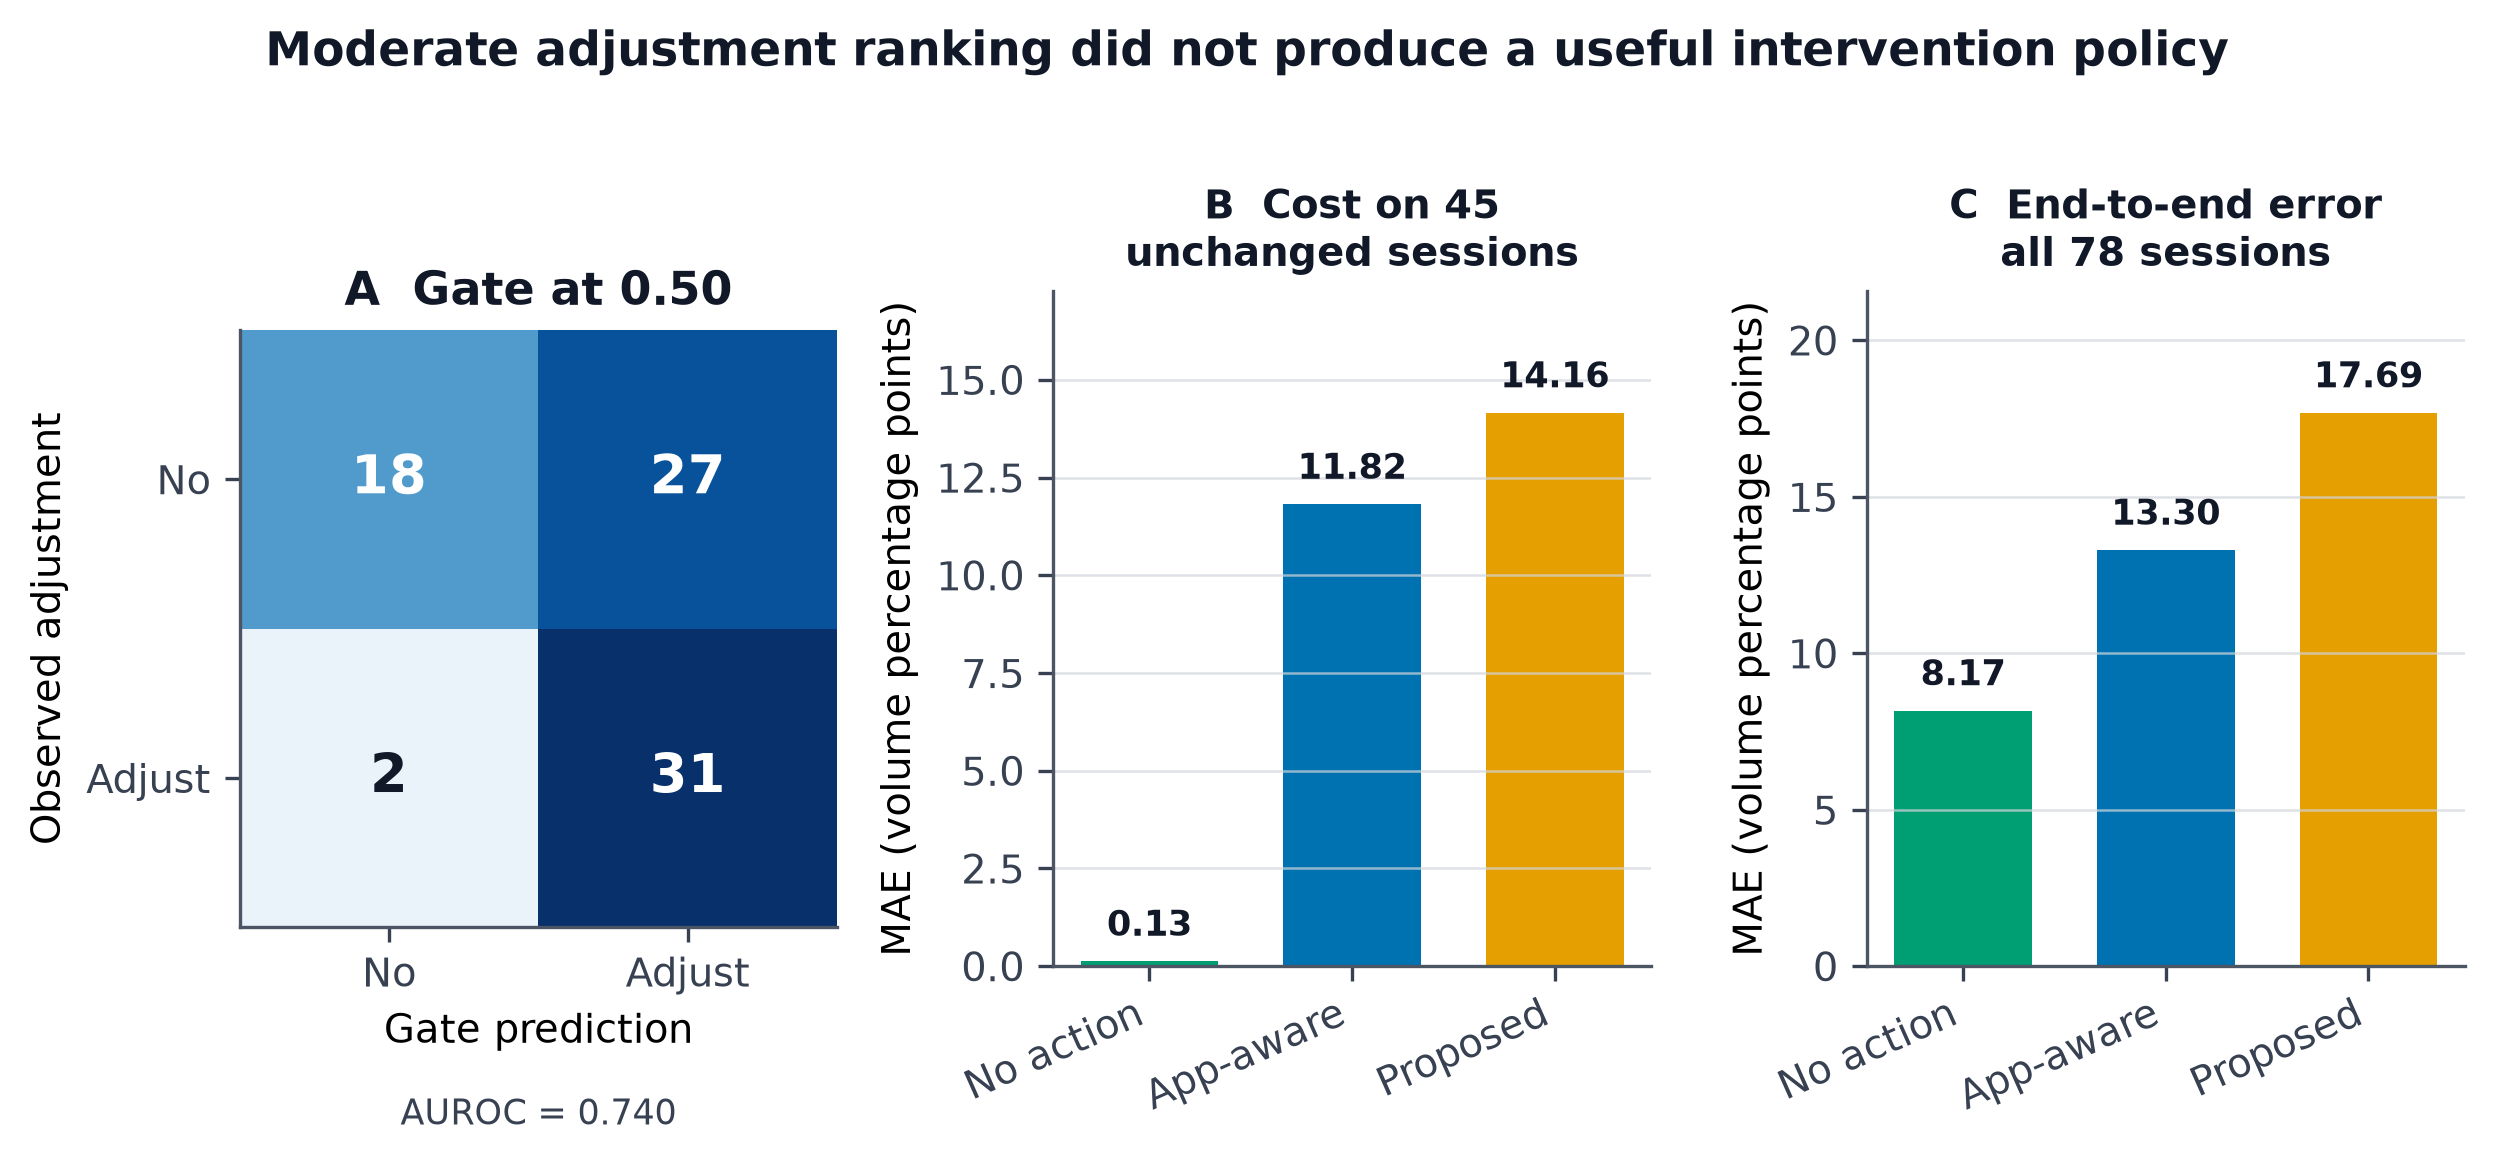
\includegraphics[width=\textwidth]{android_pilot_policy_cost.png}
\caption[Android pilot false-intervention cost]{Single-user Android pilot on 78
future sessions. Panel A shows the app-only adjustment gate at threshold 0.50.
Panel B isolates the 45 sessions with no matched adjustment: false interventions
raised MAE sharply relative to retaining the current volume. Panel C shows the same
ordering end to end. ``App-aware'' is a descriptive sensitivity; ``proposed'' is the
app-independent device/time destination policy. Exact app identities are omitted.
Lower MAE is better.}
\label{fig:android-policy-cost}
\end{figure}

\section{Interpretation and limitations}

The developmental two-stage mechanism and both observed policies are rejected on
this block. The useful methodological result is narrower: moderate ranking
performance can coexist with a harmful action policy when false positives are
costly. The appropriate comparison for an intervention is therefore not only a
classifier or destination baseline, but the utility of doing nothing.

This result comes from one author-user over 37 calendar days and 78 future test
sessions. Hardware-key adjustment is an observed action, not a direct measure of
preference, satisfaction, or intervention benefit. The mechanism was post-hoc, and
there is no cross-user, platform, clinical, or deployment evidence. A future study
would need multiple users, an independently frozen policy, and direct utility or
preference labels before testing any actuation.

\section{September saved-model follow-up (exploratory)}
\label{sec:september-volume-followup}

A separately dated follow-up used the same author-user's phone export. The September
1 file held 541 sessions; the September 15 file retained those rows unchanged and
added 110 sessions from September 2--15. The saved hybrid CatBoost object contains
a September 1 training timestamp, a 12-point discrepancy trigger, and a 0.6
correction weight. Its feature schema uses the initial volume, app, device, time,
charging/screen state, and immediately preceding-session context. Reconstructing
its predictions without refitting reproduced the later reported 24 selected
sessions and outcome metrics. The file was copied into the audit workspace on
September 15, so the internal timestamp and matching arithmetic do not independently
prove an immutable pre-September policy freeze.

Across all 110 future sessions, retaining the initial volume had MAE 9.855 and
RMSE 17.899. The saved hybrid had MAE 9.062 and RMSE 16.122, a paired MAE
improvement of 0.793 points (8.0\%). A day-clustered bootstrap over 14 dates gave
a 95\% interval $[-0.175,1.890]$ for the improvement, which includes zero.
The model changed 24 sessions. Within those sessions, MAE was 17.958 for no action
and 14.324 for the hybrid; 17 changes reduced absolute error and seven raised it.

\begin{figure}[H]
\centering
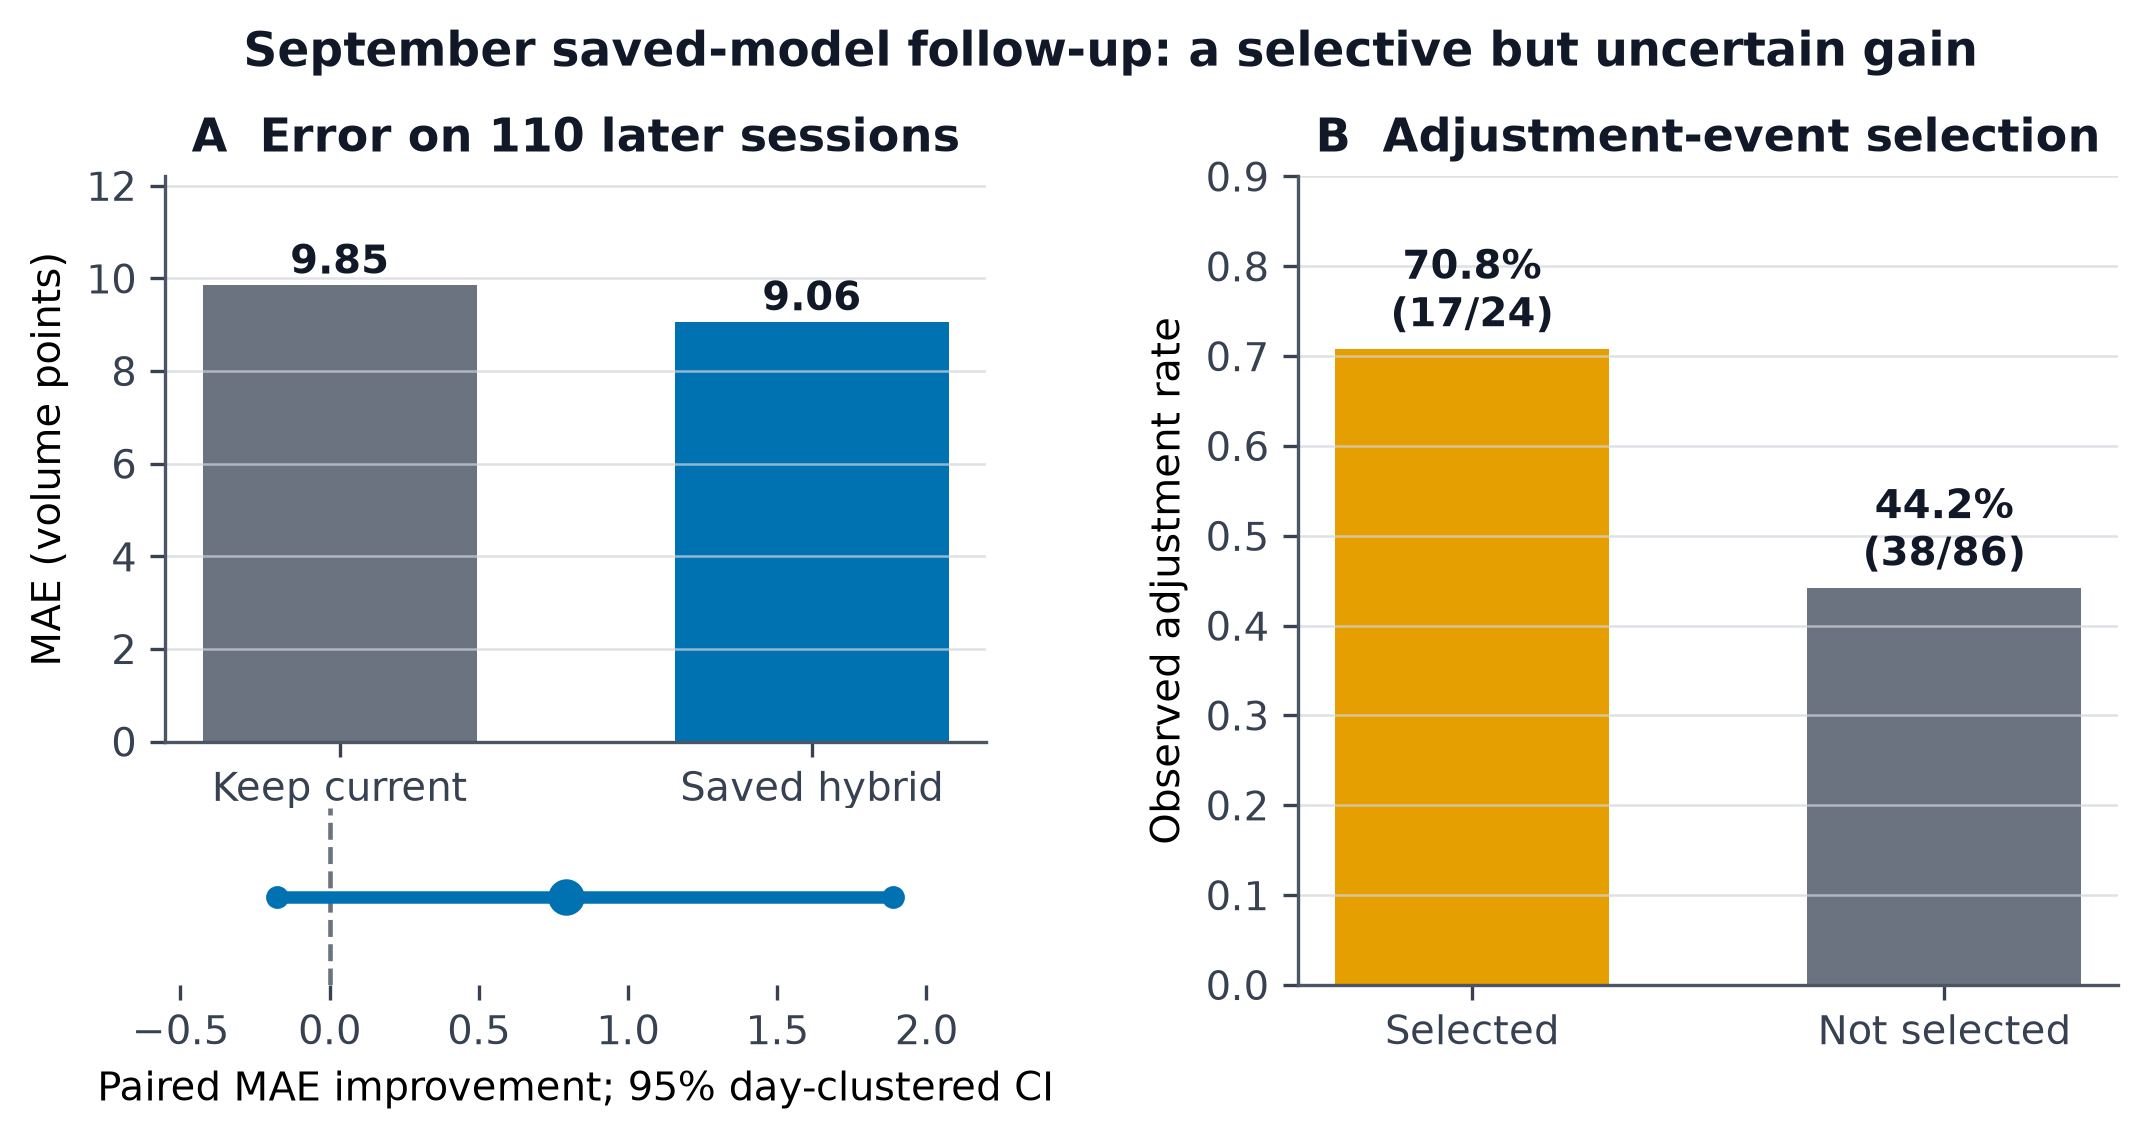
\includegraphics[width=\textwidth]{android_september_followup.png}
\caption[September saved-model volume follow-up]{Later single-user follow-up on
110 sessions from September 2--15. Panel A compares no action and the saved hybrid;
the paired MAE improvement interval crosses zero. Panel B shows observed
hardware-key adjustment rates for selected and unselected sessions. Selection is
exploratory and post-hoc, not evidence that automatic corrections were preferred.
Saved-model arithmetic was reproduced, but an immutable pre-September policy freeze
was not independently verified.}
\label{fig:android-september}
\end{figure}

\begin{table}[H]
\centering
\small
\caption[Separate Android policy evaluation blocks]{Separate single-user blocks
with different policies, not a before/after estimate for one unchanged policy.
MAE covers every session; lower is better. The September interval crosses zero.}
\label{tab:android-blocks}
\begin{tabularx}{\textwidth}{@{}L{0.31\textwidth}S[table-format=2.2]S[table-format=2.2]Y@{}}
\toprule
Block and policy & {Keep MAE} & {Policy MAE} & Interpretation \\
\midrule
Developmental test: proposed two-stage policy, 78 sessions & 8.17 & 17.69 & Policy harmed overall accuracy; 95\% paired difference versus keep: 5.31--13.49. \\
September follow-up: saved hybrid, 110 sessions & 9.85 & 9.06 & Observed 0.79-point improvement; day-clustered 95\% interval: $[-0.17,1.89]$. \\
\bottomrule
\end{tabularx}
\end{table}

The narrow positive observation is \emph{adjustment-event selection}: 17/24 selected
sessions had a hardware-key adjustment versus 38/86 unselected (70.8\% versus
44.2\%; difference 26.6 points, day-clustered 95\% interval 3.9--50.0;
uncorrected Fisher $p=0.036$). This post-hoc, uncorrected test is exploratory, not
proof that automatic correction is preferred. Six of seven selected sessions without
an observed adjustment were worsened. The earlier 78-session policy null remains;
neither Android result informs GLOBEM psychological labels or population efficacy.

\chapter{Reproducibility and Source Map}
\label{app:work-packages}

\footnotesize
\begin{longtable}{@{}L{0.18\textwidth}L{0.77\textwidth}@{}}
\caption[Work-package source map]{Compact work-package source map. GLOBEM analyses
have a runner and checked aggregate output; restricted source data are still
required for full recomputation. Android entries are aggregate-only. Exact mappings are in the
submission package's \path{CLAIM_SOURCE_MAP.md}.}
\label{tab:work-package-sources}\\
\toprule
Work package & Reproducible record and represented decision \\
\midrule
\endfirsthead
\multicolumn{2}{l}{\textit{Table \thetable\ continued}}\\
\toprule
Work package & Reproducible record and represented decision \\
\midrule
\endhead
\midrule
\multicolumn{2}{r}{\textit{Continued on next page}}\\
\endfoot
\bottomrule
\endlastfoot
RQ1 label baseline & Runner:
\path{experiments/run_label_baseline_control.py}; checked output:
\path{results/label_baseline_control/summary.json}; target prevalence extract:
\path{results/report_statistical_supplements/rq1_target_prevalence.csv}.
Represents the label-history boundary. \\
RQ1 inference & Runners in \path{experiments/run_rq1_*.py}; checked aggregates in
\path{results/rq1_clustered_inference}, \path{results/rq1_within_person_deviation},
\path{results/rq1_within_person_power_diagnostic}, and
\path{results/rq1_split_seed_sensitivity} represent clustered inference,
within-person ranking, power, and split/seed sensitivity. \\
Construct overlap & Runners: \path{experiments/run_construct_fragility_audit.py}
and \path{experiments/run_construct_overlap_sensitivity.py}; checked outputs:
\path{results/construct_fragility_audit} and
\path{results/construct_overlap_sensitivity}. Represents the redundant and
nonredundant construct-overlap audits. \\
RQ2 forecasting & Runner: \path{experiments/run_behavioural_weather_forecast.py};
checked output:
\path{results/behavioural_weather_forecast}, with the per-target reporting extract
in \path{results/report_statistical_supplements/rq2_per_target.csv} and the baseline
hierarchy in \path{results/report_statistical_supplements/rq2_baseline_summary.csv}. \\
\path{experiments/run_forecastability_phenotype.py}; checked output:
\path{results/forecastability/summary.json}. Represents
the original, subsequently rejected scalar operationalization. \\
RQ3 correction & Runnable:
\path{experiments/run_referee_robustness_checks.py}; checked output:
\path{results/referee_robustness}. Represents the construct audit,
refits, and corrected comparator-relative profile. \\
RQ4 structure & Runnable:
\path{experiments/run_structure_mechanism_followup.py} and
\path{experiments/run_profile_typology_followup.py}; checked output:
\path{results/structure_followup}. Represents profile mechanism
and typology follow-ups. \\
Personalization audit & Runnable feasibility audit:
\path{experiments/personalization/run.py}; checked output:
\path{experiments/personalization/result.json}. Represents the outcome-blind
stop before model fitting. \\
Android pilot & Privacy-safe aggregate extract:
\path{results/android_pilot/summary.json}. It verifies the displayed arithmetic and
figure, not an independent rerun from private phone logs. No deployment claim. \\
September volume follow-up & Privacy-safe aggregate extract:
\path{results/android_pilot/september_summary.json}. It represents a later,
single-user exploratory observation. The saved-model freeze was not independently
proved and the policy-improvement interval includes zero. Raw exports and predictions
stay private. \\
\end{longtable}
\normalsize

\section{Compact robustness record}

Excluding all repeat-candidate trajectories retained 232 core trajectories and a
raw fixed-model correlation of $r=0.417$ with 95\% interval $[0.261,0.562]$. This
shows that known repeats did not dominate the raw association; it does not validate
the scalar or reconstruct unique identities. In the same exclusion sample, the
standard-deviation/entropy-adjusted history-benefit profile advantages were 0.338,
0.333, and 0.242 under fixed, expanding, and disjoint regimes (all $p=0.002$).
The sequence controls were based on short discretized records (median 68 observed
days) and remain descriptive. H3 was inconclusive because its approximate corrected
80\% minimum detectable $|r|$ was 0.172. The post-hoc distress estimates were
heterogeneous across cohorts and do not support distress prediction or within-person
change detection.

\section{Canonical build and analysis command}

From \texttt{deliverables/tuhh\_project\_report/}:

\begin{verbatim}
python3.11 -m venv .report-venv
.report-venv/bin/pip install -r requirements-report.txt
MPLBACKEND=Agg .report-venv/bin/python make_figures.py
tectonic main.tex
\end{verbatim}

From the repository root:

\begin{verbatim}
python3.11 -m venv .analysis-venv
.analysis-venv/bin/pip install -e .
.analysis-venv/bin/python scripts/run_rq1_clustered_inference.py
.analysis-venv/bin/python scripts/run_rq1_within_person_deviation.py
.analysis-venv/bin/python scripts/run_rq1_within_person_power_diagnostic.py
.analysis-venv/bin/python scripts/run_rq1_split_seed_sensitivity.py
.analysis-venv/bin/python scripts/run_construct_overlap_sensitivity.py
.analysis-venv/bin/python scripts/build_report_statistical_supplements.py
\end{verbatim}

\clearpage
\chapter*{Declaration of Independent Work}
\phantomsection
\addcontentsline{toc}{chapter}{Declaration of Independent Work}
\thispagestyle{plain}

I hereby declare that I prepared this report independently and used no sources or
aids other than those identified in the report. All passages, data, and ideas taken
directly or indirectly from other sources are marked as such and attributed to their
sources. Any use of AI-assisted tools is disclosed in the Data and Code Availability
statement. I reviewed the submitted analyses, code, figures, citations, and text and
accept responsibility for the content of this work.

\vfill
\noindent
\begin{tabularx}{\textwidth}{@{}X@{\hspace{2cm}}X@{}}
\rule{\linewidth}{0.4pt} & \rule{\linewidth}{0.4pt} \\
Place and date & Signature \\
\end{tabularx}

\clearpage
\end{document}
